% =====================================================================
%  A Practical Workshop on Column Generation and Branch-and-Price
%  4-hour workshop, intended for Master/PhD OR students
%  Author: built for Polytechnique Montreal workshop
% =====================================================================
\documentclass[10pt,aspectratio=169]{beamer}

% --- Theme -----------------------------------------------------------
\usetheme{metropolis}
\usecolortheme{default}
\metroset{progressbar=frametitle, sectionpage=progressbar, subsectionpage=progressbar}
% Custom frame numbering "k / N" using the real total, with author tag
\setbeamertemplate{frame numbering}{%
  \insertshortauthor \;|\; \insertframenumber\,/\,\inserttotalframenumber}

% --- Packages --------------------------------------------------------
\usepackage[utf8]{inputenc}
\usepackage[T1]{fontenc}
\usepackage{amsmath,amssymb,mathtools}
\usepackage{tikz}
\usepackage{tcolorbox}
\usepackage{qrcode}                            % title-page QR
% Workshop URL embedded by the QR code (edit me if the deliverable moves).
\newcommand{\workshopURL}{https://github.com/legraina/workshop-cg}
\usepackage{booktabs}
\usepackage{listings}
\usepackage{xcolor}
\usepackage{array}
\usetikzlibrary{positioning,arrows.meta,shapes.geometric,calc,fit,backgrounds,decorations.pathreplacing}

\tcbuselibrary{skins,breakable}

% --- Colors ----------------------------------------------------------
\definecolor{accent}{HTML}{C72A2A}
\definecolor{accent2}{HTML}{1F6FB2}
\definecolor{soft}{HTML}{F2F2F2}
\definecolor{codebg}{HTML}{F7F7F7}
\definecolor{codekw}{HTML}{0033B3}
\definecolor{codestr}{HTML}{067D17}
\definecolor{codecom}{HTML}{8C8C8C}

% --- Listings (Python) -----------------------------------------------
\lstdefinestyle{py}{
  language=Python,
  basicstyle=\ttfamily\scriptsize,
  keywordstyle=\color{codekw}\bfseries,
  stringstyle=\color{codestr},
  commentstyle=\color{codecom}\itshape,
  showstringspaces=false,
  breaklines=true,
  backgroundcolor=\color{codebg},
  frame=single,
  rulecolor=\color{black!20},
  numbers=none,
  xleftmargin=4pt,
  xrightmargin=4pt,
  framexleftmargin=2pt,
  framexrightmargin=2pt,
  aboveskip=2pt,
  belowskip=2pt,
}
\lstset{style=py}

% --- Custom pseudocode (no algpseudocode available) ------------------
\newcounter{algoline}
\newenvironment{algo}[1][Algorithm]{%
  \setcounter{algoline}{0}%
  \begin{tcolorbox}[colback=soft,colframe=accent2!70,sharp corners,
      boxrule=0.4pt,left=4pt,right=4pt,top=2pt,bottom=2pt,
      title=\textbf{#1}]%
  \ttfamily\small
  \begin{list}{\stepcounter{algoline}\textcolor{accent2}{\scriptsize\arabic{algoline}:}}%
    {\setlength{\leftmargin}{2.0em}\setlength{\itemsep}{0.1em}\setlength{\topsep}{0pt}}%
}{%
  \end{list}\end{tcolorbox}%
}
\newcommand{\Indent}{\hspace*{1.2em}}
\newcommand{\IndentTwo}{\hspace*{2.4em}}

% --- Math shortcuts --------------------------------------------------
\newcommand{\R}{\mathbb{R}}
\newcommand{\Z}{\mathbb{Z}}
\newcommand{\N}{\mathbb{N}}
\newcommand{\transpose}{^{\!\top}}
\DeclareMathOperator*{\argmin}{arg\,min}
\DeclareMathOperator*{\argmax}{arg\,max}
\newcommand{\rmp}{\mathsf{RMP}}
\newcommand{\masterp}{\mathsf{MP}}
\newcommand{\sub}{\mathsf{SP}}
\newcommand{\redcost}{\bar{c}}
\newcommand{\dual}[1]{\boldsymbol{\pi}_{#1}}

% --- Boxes -----------------------------------------------------------
\newtcolorbox{keybox}[1][Key idea]{
  colback=accent!8,colframe=accent,sharp corners,
  boxrule=0.5pt, left=4pt,right=4pt,top=3pt,bottom=3pt,
  fonttitle=\bfseries, title={#1}}

\newcommand{\cmark}{{\color{green!50!black}\ensuremath{\checkmark}}}
\newcommand{\xmark}{{\color{red!70!black}\ensuremath{\times}}}

\newtcolorbox{warnbox}[1][Pitfall]{
  colback=yellow!10,colframe=orange!80!black,sharp corners,
  boxrule=0.5pt,left=4pt,right=4pt,top=3pt,bottom=3pt,
  fonttitle=\bfseries,title={#1}}

\newtcolorbox{exbox}[1][Hands-on exercise]{
  colback=green!5,colframe=green!50!black,sharp corners,
  boxrule=0.5pt,left=4pt,right=4pt,top=3pt,bottom=3pt,
  fonttitle=\bfseries\sffamily,title={\textbf{[lab]}\; #1}}

% --- Title -----------------------------------------------------------
\title{Column Generation \& Branch-and-Price}
\subtitle{Theory deck -- a 4-hour practical workshop\\ \small{Modeling -- Pricing -- Integrality -- Optimality}}
\author{Antoine Legrain}
\institute{Polytechnique Montr\'eal}
\date{\today}

\begin{document}

% =====================================================================
%  Title and outline
% =====================================================================
\begin{frame}
  \titlepage
  \begin{tikzpicture}[remember picture, overlay]
    \node[anchor=south east, xshift=-60mm, yshift=8mm]
          at (current page.south east)
          {\begin{tikzpicture}
             \node[fill=white, draw=black!15, line width=0.4pt,
                   inner sep=4pt, rounded corners=2pt]
               {\qrcode[height=3cm]{\workshopURL}};
           \end{tikzpicture}};
    \node[anchor=south east, xshift=-62mm, yshift=4mm,
          font=\scriptsize\itshape, text=black!70]
          at (current page.south east)
          {scan for the workshop kit};
  \end{tikzpicture}
\end{frame}

\begin{frame}{What you will leave the room with}
  By the end of these four hours you should be able to
  \begin{itemize}\setlength{\itemsep}{2pt}
    \item Recognise problems that admit an extended formulation with
          \alert{exponentially many variables} (routes, patterns, schedules, \dots).
    \item Build the \alert{master/pricing} pair and run a column-generation loop.
    \item Write the pricing problem as a \alert{Resource-Constrained Shortest Path}
          (RCSPP) and call a labelling algorithm.
    \item Apply the standard \alert{efficiency tricks}: multiple columns, heuristic
          pricing, stabilization, tailing-off.
    \item Recover an integer solution either heuristically (RMP-MIP, diving) or
          exactly with \alert{branch-and-price}, including the
          \alert{Lagrangian bound}.
    \item Implement and debug the loop on a VRPTW instance with
          HiGHS + the \texttt{rcspp} package.
  \end{itemize}
\end{frame}

\begin{frame}{4-hour outline}
  \small
  \begin{tabular}{@{}lll@{}}
    \toprule
    Time & Topic & Block \\
    \midrule
    00:00--00:30 & Why column generation? & Part 1 -- Motivation \\
    00:30--01:15 & The CG mechanics, RMP \& pricing & Part 2 -- Mechanics \\
    01:15--02:00 & The pricing subproblem (RCSPP) & Part 3 -- RCSPP \\
    \midrule
    \multicolumn{3}{c}{\emph{15-minute break}} \\
    \midrule
    02:15--02:45 & Making CG fast & Part 4 -- Implementation \\
    02:45--03:15 & From LP to integer (heuristics) & Part 5 -- IP heuristics \\
    03:15--03:50 & Branch-and-price for optimality & Part 6 -- B\&P \\
    03:50--04:00 & VRPTW illustration / lab kickoff & Part 7 -- Code \\
    \bottomrule
  \end{tabular}
  \vspace{0.5em}
  \begin{itemize}\small
    \item Hands-on coding alternates with the slides during Parts 3, 5 and 7.
  \end{itemize}
\end{frame}

\begin{frame}{Scope and non-scope}
  \begin{columns}[T,onlytextwidth]
    \column{0.48\textwidth}
    \textbf{Inside the scope}
    \begin{itemize}\small
      \item Modelling with a \alert{set-partitioning / set-covering} master.
      \item Pricing as a \alert{shortest path with resources}.
      \item Stabilisation, heuristic pricing, multi-column.
      \item Diving \& restricted master heuristic.
      \item Branching rules that do \alert{not} kill the pricer.
      \item The \alert{Lagrangian bound} for early termination.
    \end{itemize}
    \column{0.48\textwidth}
    \textbf{Outside the scope}
    \begin{itemize}\small
      \item Full Dantzig--Wolfe / Lagrangian \emph{theory}
            (we keep an executive summary at the end of Part 2).
      \item Cut-and-price (a.k.a.\ branch-cut-and-price) -- mentioned, not derived.
      \item GPU pricing / parallel B\&P.
      \item Stochastic or robust extensions.
    \end{itemize}
  \end{columns}
  \vfill
  \begin{keybox}[Reference for the curious]
    J.~Desrosiers, M.~L\"ubbecke, G.~Desaulniers \& J.B.~Gauthier,
    \emph{Branch-and-Price}, Springer, 2026 (ISBN 978-3-031-96917-1, open
    access, the PDF in your folder) covers everything we skip -- in
    particular cut-and-price, stabilisation theory and computational case
    studies.
  \end{keybox}
\end{frame}

% =====================================================================
\section{Part 1 -- Why column generation?}
% =====================================================================

\begin{frame}{The problem we want to solve}
  Generic combinatorial optimization problem
  \[
     \min \; c\transpose x \quad \text{s.t.}\quad Ax \ge b,\quad x\in X
  \]
  where $X$ encodes \alert{combinatorial structure} (knapsack, paths, schedules\dots).

  \medskip

  Two ways to write it as a (mixed-)integer linear program.
  \begin{columns}[T,onlytextwidth]
    \column{0.48\textwidth}
    \textbf{Compact (arc-flow) formulation}
    \begin{itemize}\small
      \item Variables = ``physical'' decisions (use arc, assign job\dots).
      \item Polynomial number of vars and constraints.
      \item LP relaxation is often \alert{very weak}.
    \end{itemize}
    \column{0.48\textwidth}
    \textbf{Extended (path-flow) formulation}
    \begin{itemize}\small
      \item Variable per \alert{combinatorial object} (route, pattern, roster).
      \item Possibly $\sim\!10^{20}$ variables.
      \item LP relaxation is often \alert{much tighter}.
    \end{itemize}
  \end{columns}
  \vfill
  Column generation lets us \alert{never write down} the extended formulation.
\end{frame}

\begin{frame}{Motivating example 1 -- 1D Cutting Stock}
  Rolls of width $W$ must be cut to satisfy demand $d_i$ of width $w_i$.
  \begin{center}
  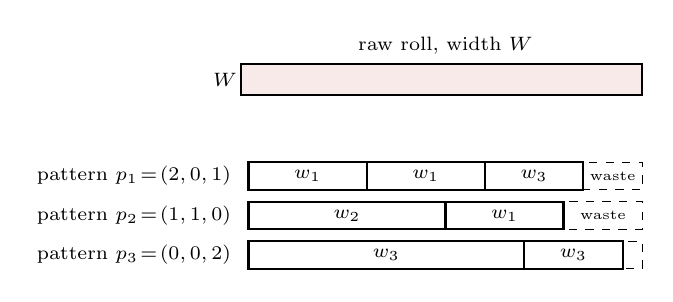
\begin{tikzpicture}[scale=0.5,every node/.style={font=\scriptsize}]
    % Source roll
    \draw[thick,fill=accent!10] (-0.2,1.4) rectangle (10,2.2);
    \node at (-0.6,1.8) {$W$};
    \node[above] at (5,2.2) {raw roll, width $W$};
    % Patterns
    \begin{scope}[yshift=-1.0cm]
      \draw[thick] (0,0) rectangle (3,0.7); \draw[thick] (3,0) rectangle (6,0.7);
      \draw[thick] (6,0) rectangle (8.5,0.7); \draw[dashed] (8.5,0) rectangle (10,0.7);
      \node at (1.5,0.35){$w_1$};\node at (4.5,0.35){$w_1$};\node at (7.25,0.35){$w_3$};
      \node at (9.25,0.35){\tiny waste};
      \node[left] at (-0.2,0.35) {pattern $p_1\!=\!(2,0,1)$};
    \end{scope}
    \begin{scope}[yshift=-2.0cm]
      \draw[thick] (0,0) rectangle (5,0.7); \draw[thick] (5,0) rectangle (8,0.7);
      \draw[dashed] (8,0) rectangle (10,0.7);
      \node at (2.5,0.35){$w_2$};\node at (6.5,0.35){$w_1$};
      \node at (9,0.35){\tiny waste};
      \node[left] at (-0.2,0.35) {pattern $p_2\!=\!(1,1,0)$};
    \end{scope}
    \begin{scope}[yshift=-3.0cm]
      \draw[thick] (0,0) rectangle (7,0.7); \draw[thick] (7,0) rectangle (9.5,0.7);
      \draw[dashed] (9.5,0) rectangle (10,0.7);
      \node at (3.5,0.35){$w_3$};\node at (8.25,0.35){$w_3$};
      \node[left] at (-0.2,0.35) {pattern $p_3\!=\!(0,0,2)$};
    \end{scope}
  \end{tikzpicture}
  \end{center}
  \textbf{Pattern formulation (Gilmore--Gomory, 1961).} $a_{ip}=$ \# items $i$
  in pattern $p$, with $\sum_i w_i a_{ip}\!\le\!W$. Variable $x_p\!\ge\!0$ =
  ``how many rolls cut according to $p$''.
  \[
     \min \!\!\sum_{p\in\mathcal P} \!x_p \;\;\text{s.t.}\;\;
       \!\!\sum_{p\in\mathcal P}\! a_{ip} x_p \ge d_i \;\forall i,\;
       x_p\in\Z_+ .
  \]
  The LP relaxation is empirically very tight (often within 1 unit of the IP
  optimum on 1D cutting-stock). We \alert{generate} $\mathcal P$ on demand.
\end{frame}

\begin{frame}{Motivating example 2 -- VRPTW}
  Customers $\mathcal N$ with demand $q_i$, window $[a_i,b_i]$, depot $0$,
  fleet of capacity $Q$.
  \begin{columns}[T,onlytextwidth]
    \column{0.42\textwidth}
    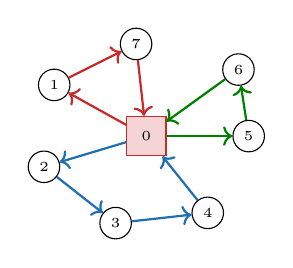
\begin{tikzpicture}[scale=0.65,every node/.style={font=\tiny}]
      \tikzstyle{c}=[circle,draw,minimum size=4mm,inner sep=0pt,fill=white];
      \tikzstyle{d}=[rectangle,draw,minimum size=5mm,inner sep=0pt,
                     fill=accent!20,draw=accent];
      \node[d] (0)  at (0,0)   {0};
      \node[c] (1) at (-1.8,1.0)  {1};
      \node[c] (2) at (-2.0,-0.6) {2};
      \node[c] (3) at (-0.6,-1.7) {3};
      \node[c] (4) at (1.2,-1.5)  {4};
      \node[c] (5) at (2.0,0.0)   {5};
      \node[c] (6) at (1.8,1.3)   {6};
      \node[c] (7) at (-0.2,1.8)  {7};
      \draw[->,accent,thick]         (0)--(1); \draw[->,accent,thick]   (1)--(7); \draw[->,accent,thick]   (7)--(0);
      \draw[->,accent2,thick]        (0)--(2); \draw[->,accent2,thick]  (2)--(3);
      \draw[->,accent2,thick]        (3)--(4); \draw[->,accent2,thick]  (4)--(0);
      \draw[->,green!50!black,thick] (0)--(5); \draw[->,green!50!black,thick] (5)--(6);
      \draw[->,green!50!black,thick] (6)--(0);
    \end{tikzpicture}
    \column{0.55\textwidth}
    \small
    A \emph{route} $p$ = a feasible depot-to-depot tour visiting
    $S_p\subseteq\mathcal N$ inside capacity and windows.\;\;Cost $c_p$ =
    total distance.\;\;3 coloured routes shown $=$ 3 columns of the master.
  \end{columns}
  \[\textstyle
    \min \!\sum_{p\in\mathcal P} c_p\, x_p \;\;\text{s.t.}\;\;
       \!\sum_{p\in\mathcal P}\!a_{ip}\,x_p = 1\;\forall i\!\in\!\mathcal N,\;
       x_p\!\ge\!0,\; a_{ip}\!=\!\mathbf 1[i\!\in\! S_p].
  \]
  Capacity \& windows are pushed \emph{inside} $\mathcal P$. $|\mathcal P|>10^{20}$ on Solomon-100.
\end{frame}

\begin{frame}{Why is the extended LP tighter?}
  \begin{columns}[T,onlytextwidth]
    \column{0.50\textwidth}
    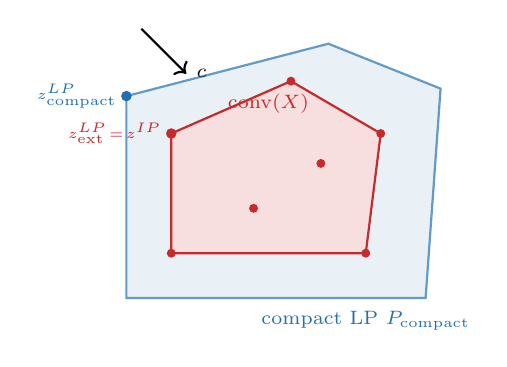
\begin{tikzpicture}[scale=0.95,every node/.style={font=\scriptsize}]
      % Compact LP relaxation (large polytope)
      \filldraw[fill=accent2!10,draw=accent2!70,thick]
         (-0.2,-0.2) -- (3.8,-0.2) -- (4.0,2.6) -- (2.5,3.2) -- (-0.2,2.5) -- cycle;
      % Convex hull of integer points (smaller, inside)
      \filldraw[fill=accent!15,draw=accent,thick]
         (0.4,0.4) -- (3.0,0.4) -- (3.2,2.0) -- (2.0,2.7) -- (0.4,2.0) -- cycle;
      % Integer points
      \foreach \p in {(0.4,0.4),(3.0,0.4),(3.2,2.0),(2.0,2.7),(0.4,2.0),(1.5,1.0),(2.4,1.6)} {
         \fill[accent] \p circle (1.7pt);
      }
      % Objective direction
      \draw[->,thick,black] (0.0,3.4) -- (0.6,2.8) node[right]{$c$};
      % Labels
      \node[accent2] at (3.0,-0.5) {compact LP $P_{\text{compact}}$};
      \node[accent] at (1.7,2.4) {conv$(X)$};
      % LP optimum on outer
      \fill[accent2] (-0.2,2.5) circle (2.0pt);
      \node[accent2,left] at (-0.2,2.5) {\tiny $z^{LP}_{\text{compact}}$};
      % LP optimum on inner = integer optimum
      \fill[accent] (0.4,2.0) circle (2.0pt);
      \node[accent,left] at (0.4,2.0) {\tiny $z^{LP}_{\text{ext}}\!=\!z^{IP}$};
    \end{tikzpicture}
    \column{0.48\textwidth}
    \small
    The extended-formulation polytope is exactly $\text{conv}(X)$: the convex
    hull of the integer feasible objects (routes, patterns).
    \medskip

    The compact LP is some \alert{outer} relaxation of the same set --
    enlarged by all the convex combinations that the linking variables admit.
    \medskip

    \begin{itemize}\scriptsize
      \item Extended LP $\le$ compact LP for any objective.
      \item Strict inequality whenever $X$ has the \alert{non-integer
            extreme points} that we have been hiding inside the pricer.
    \end{itemize}
  \end{columns}

  \vspace{0.3em}
  \begin{keybox}[Concretely on VRPTW Solomon]
    Compact LP $\approx 60\%$ of optimum; set-partitioning LP $\approx 99\%$.
    The difference between a 3-day B\&C run and a 30-second B\&P run.
  \end{keybox}
\end{frame}

\begin{frame}{Other classical applications}
  \begin{itemize}\setlength{\itemsep}{4pt}
    \item \textbf{Crew scheduling / pairing} -- columns are legal duties;
          pricing is a constrained shortest path on a flight network.
    \item \textbf{Nurse / employee rostering} -- columns are individual rosters
          honouring labour rules.
    \item \textbf{Bin packing, multi-knapsack} -- columns are packings.
    \item \textbf{Vehicle routing} (CVRP, VRPTW, PDPTW, DARP) -- columns are routes.
    \item \textbf{Multi-commodity flow} -- columns are paths per commodity.
    \item \textbf{Lot-sizing, network design, unit commitment} -- columns are
          per-machine production plans / on-off schedules.
    \item \textbf{Graph colouring} -- columns are independent sets.
  \end{itemize}
  \vfill
  \begin{keybox}[Pattern]
    Whenever your problem looks like ``assemble a global plan from many
    \emph{individually feasible} sub-plans'', think column generation.
  \end{keybox}
\end{frame}

\begin{frame}{When NOT to use column generation}
  \begin{itemize}
    \item Compact LP relaxation is already close to optimum.
    \item No nice combinatorial structure in $X$ (pricing problem is hopeless).
    \item Few enough columns that branch-and-cut handles them.
    \item You need fast \emph{re-optimisation} after small data perturbations
          (CG warm-starts can be tricky -- but possible).
  \end{itemize}
  \vspace{0.5em}
  \begin{warnbox}[Honest warning]
    CG is software-engineering heavy: master + pricer + branching + bounding +
    column pool management. A toy implementation in Python is doable in
    300 lines (we will see); a competitive one is thousands.
  \end{warnbox}
\end{frame}

% =====================================================================
\section{Part 2 -- The CG mechanics}
% =====================================================================

\begin{frame}{The master problem (MP)}
  Generic LP with possibly exponentially many variables:
  \[
    (\masterp)\quad
    z^* \;=\; \min_{x\ge 0}\;\sum_{p\in\mathcal P} c_p\, x_p
    \quad\text{s.t.}\quad
    \sum_{p\in\mathcal P} \mathbf a_p\, x_p \ge \mathbf b
  \]
  with $\mathbf a_p\in\R^m$, $c_p\in\R$, $|\mathcal P|$ huge.

  \medskip
  \textbf{Restricted master ($\rmp$).} Pick a small $\widetilde{\mathcal P}\subseteq\mathcal P$
  containing at least one feasible point and solve
  \[
     z^{\rmp} \;=\; \min_{x\ge 0}\;\sum_{p\in\widetilde{\mathcal P}} c_p\, x_p
     \quad\text{s.t.}\quad
     \sum_{p\in\widetilde{\mathcal P}} \mathbf a_p\, x_p \ge \mathbf b .
  \]

  Clearly $z^{\rmp}\ge z^*$. We will iteratively add columns and tighten.
\end{frame}

\begin{frame}{The basic loop, in one slide}
  \begin{columns}[T,onlytextwidth]
    \column{0.55\textwidth}
    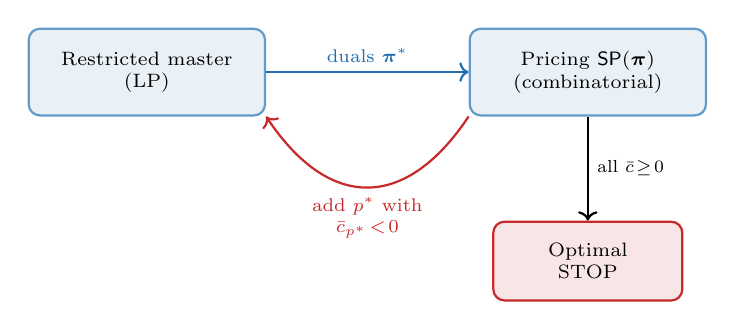
\begin{tikzpicture}[every node/.style={font=\scriptsize}]
      \tikzstyle{box}=[rounded corners,draw,minimum width=30mm,minimum height=11mm,
                       align=center,fill=accent2!10,draw=accent2!70,thick];
      \tikzstyle{stop}=[rounded corners,draw,minimum width=24mm,minimum height=10mm,
                       align=center,fill=accent!12,draw=accent,thick];
      \node[box]  (rmp) at (0,0)    {Restricted master\\(LP)};
      \node[box]  (sub) at (5.6,0)  {Pricing $\sub(\boldsymbol\pi)$\\(combinatorial)};
      \node[stop] (stop) at (5.6,-2.4) {Optimal\\STOP};
      \draw[->,thick,accent2] (rmp.east) -- node[above,scale=0.95]{duals $\boldsymbol\pi^*$} (sub.west);
      \draw[->,thick,accent]  (sub.south west)
           .. controls +(-0.8,-1.2) and +(0.8,-1.2) ..
           node[below,align=center,scale=0.95]{add $p^*$ with\\$\redcost_{p^*}\!<\!0$}
           (rmp.south east);
      \draw[->,thick] (sub.south) -- node[right,scale=0.9]{all $\redcost\!\ge\!0$} (stop.north);
    \end{tikzpicture}
    \column{0.42\textwidth}
    \small
    \begin{enumerate}\setlength{\itemsep}{2pt}
      \item Solve $\rmp$ $\to$ primal $\bar x$, duals $\boldsymbol\pi^*$.
      \item Find $p^*$ with $\redcost_{p^*}<0$.
      \item Else $\bar x$ optimal for $\masterp$.
    \end{enumerate}
  \end{columns}
  \medskip
  \begin{keybox}[Reduced cost of column $p$]
    \[
       \redcost_p \;=\; c_p \;-\; \boldsymbol\pi^{*\top}\mathbf a_p
                   \;=\; c_p \;-\; \sum_{i}\!\pi^*_i\, a_{ip}.
    \]
    A column with $\redcost_p<0$ is \alert{undervalued} by the current
    duals -- bringing it into the basis improves the LP.
  \end{keybox}
\end{frame}

\begin{frame}{Reduced cost \& optimality}
  \begin{columns}[T,onlytextwidth]
    \column{0.48\textwidth}
    \textbf{Primal} ($\rmp$ over $\widetilde{\mathcal P}$)
    \begin{align*}
      \min\;& \sum_{p\in\widetilde{\mathcal P}} c_p\, x_p \\
      \text{s.t.}\;& \sum_{p\in\widetilde{\mathcal P}} \mathbf a_p\, x_p \;\ge\; \mathbf b
                     \quad [\boldsymbol\pi]\\
      & x_p \ge 0 \;\;\forall p
    \end{align*}
    \column{0.48\textwidth}
    \textbf{Dual}
    \begin{align*}
      \max\;& \boldsymbol\pi^{\!\top} \mathbf b \\
      \text{s.t.}\;& \boldsymbol\pi^{\!\top} \mathbf a_p \;\le\; c_p
                     \;\;\forall p\in\widetilde{\mathcal P} \\
      & \boldsymbol\pi \ge \mathbf 0
    \end{align*}
  \end{columns}
  \medskip

  Each dual feasibility constraint is exactly $\redcost_p\ge 0$ with
  $\redcost_p = c_p - \boldsymbol\pi^{\!\top}\mathbf a_p$.
  \begin{itemize}\small
    \item If $\redcost_p\ge 0$ for \alert{all} $p\in\mathcal P$ (not just in
          $\widetilde{\mathcal P}$), then $\boldsymbol\pi^*$ is dual feasible
          for $\masterp$ and $\bar x$ is primal optimal -- $\masterp$ optimum
          reached.
    \item If some $\redcost_p<0$, the dual constraint is violated by $p$:
          add $p$ to $\widetilde{\mathcal P}$ and iterate.
  \end{itemize}
  Searching for violated dual constraints is the pricing problem $\sub$:
  $\min_{p\in\mathcal P} \big\{c_p - \boldsymbol\pi^{*\top}\mathbf a_p\big\}$.
\end{frame}

\begin{frame}{Why ``column'' generation?}
  Imagine writing the (huge) constraint matrix $A$ explicitly:
  \[
    A = \big[\, \mathbf a_{p_1}\;\,\mathbf a_{p_2}\;\,\cdots\;\,\mathbf a_{p_K}\,\big],\qquad
    K=|\mathcal P|.
  \]
  The simplex method \emph{prices} non-basic variables one by one until it
  finds one with negative reduced cost. CG just outsources that pricing to a
  combinatorial oracle:
  \begin{center}
  \begin{tabular}{@{}lcl@{}}
    \toprule
    & Standard simplex pricing & Column generation \\
    \midrule
    Where & explicit columns & $\mathcal P$ implicit \\
    Cost & $O(|\mathcal P|)$ scan & solve $\sub(\boldsymbol\pi)$ \\
    Output & one entering col. & one (or many) col. \\
    Stop  & all $\redcost\ge 0$ & all $\redcost\ge 0$ \\
    \bottomrule
  \end{tabular}
  \end{center}
\end{frame}

\begin{frame}{\textbf{[ask the room]} What is the pricer for cutting stock?}
  Master $\min\sum_p x_p$ s.t.\ $\sum_p a_{ip} x_p \ge d_i$, with dual
  $\pi_i\!\ge\!0$ on each demand row.

  \medskip
  \begin{keybox}[Question for the audience]
    A column $p$ here is a cutting pattern $a_p\!\in\!\Z_+^I$ with
    $\sum_i w_i a_{ip}\!\le\!W$.\;\;Its master cost is $c_p\!=\!1$.
    \begin{itemize}
      \item Write the reduced cost $\redcost_p$ of pattern $p$.
      \item For fixed duals $\boldsymbol\pi$, what classic combinatorial
            problem do you minimise to find the most negative $\redcost_p$?
    \end{itemize}
  \end{keybox}
  \medskip
  \emph{Take a minute, then we move to the next slide for the answer.}
\end{frame}

\begin{frame}{Pricing for the pattern formulation (cutting stock)}
  Master $\min\sum_p x_p$ s.t.\ $\sum_p a_{ip}x_p\ge d_i$, dual
  $\pi_i\!\ge\!0$ on each demand constraint. Reduced cost
  $\redcost_p = 1 - \sum_i \pi_i\, a_{ip}.$
  Pricing = \alert{integer knapsack}
  $\;\max_{a\in\Z_+^I}\sum_i \pi_i a_i$ s.t.\ $\sum_i w_i a_i\le W$.
  \begin{center}
  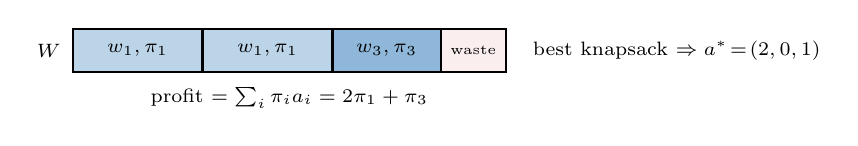
\begin{tikzpicture}[scale=0.55,every node/.style={font=\scriptsize}]
    \draw[thick,fill=accent!8] (0,0) rectangle (10,1.0);
    \node[left] at (-0.05,0.5) {$W$};
    \draw[fill=accent2!30,thick] (0,0)   rectangle (3,1.0);   \node at (1.5,0.5){$w_1,\pi_1$};
    \draw[fill=accent2!30,thick] (3,0)   rectangle (6,1.0);   \node at (4.5,0.5){$w_1,\pi_1$};
    \draw[fill=accent2!50,thick] (6,0)   rectangle (8.5,1.0); \node at (7.25,0.5){$w_3,\pi_3$};
    \draw[dashed] (8.5,0) rectangle (10,1.0); \node at (9.25,0.5){\tiny waste};
    \node[right] at (10.4,0.5) {best knapsack $\Rightarrow a^*\!=\!(2,0,1)$};
    \node at (5,-0.6) {profit $= \sum_i \pi_i a_i = 2\pi_1+\pi_3$};
  \end{tikzpicture}
  \end{center}
  \begin{itemize}\small
    \item If profit $> 1$: pattern $a^*$ has $\redcost_{p^*}<0$, add it to $\rmp$.
    \item If profit $\le 1$: \alert{no} pattern improves $\rmp$ -- LP optimum.
  \end{itemize}
\end{frame}

\begin{frame}{\textbf{[ask the room]} What is the pricer for VRPTW?}
  Master $\min\sum_p c_p x_p$ s.t.\ $\sum_p a_{ip}x_p=1$, duals
  $\pi_i\!\in\!\R$.\;A column is a feasible route
  $p=(0,i_1,\dots,i_k,0)$, with $c_p=\sum_{(u,v)\in p}d_{uv}$.

  \medskip
  \begin{keybox}[Question for the audience]
    \begin{itemize}
      \item Write $\redcost_p$ as a sum over the arcs of the route.
      \item What is the resulting pricing problem on the customer
            graph? How is it different from a classical shortest path?
    \end{itemize}
  \end{keybox}
  \medskip
  \emph{Hint: think about what the duals $\pi_v$ ``pay'' along the route.}
\end{frame}

\begin{frame}{Pricing for the set-partitioning master (VRPTW)}
  Master $\min\sum_p c_p x_p$ s.t.\ $\sum_p a_{ip}x_p=1$, duals $\pi_i\!\in\!\R$.
  A route $p=(0,i_1,\dots,i_k,0)$ has $c_p=\sum_{(u,v)\in p} d_{uv}$ and visits
  $S_p$, so
  \[
    \redcost_p = c_p - \sum_{i\in S_p}\!\pi_i
               = \sum_{(u,v)\in p}\!\big(d_{uv}-\pi_v\big),\;\pi_0\!:=\!0.
  \]
  Pricing = \alert{shortest depot-to-depot path} on the graph with arc cost
  $\bar d_{uv}=d_{uv}-\pi_v$, subject to capacity \& time windows: \alert{RCSPP}.
  \begin{center}
  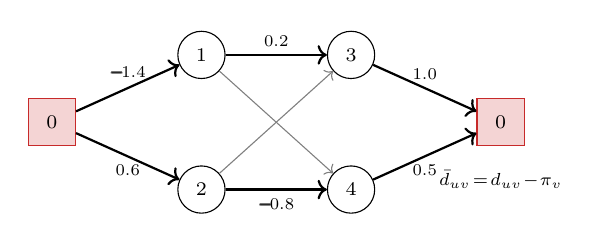
\begin{tikzpicture}[every node/.style={font=\scriptsize},scale=0.95]
    \tikzstyle{c}=[circle,draw,minimum size=6mm,inner sep=0pt,fill=white];
    \tikzstyle{d}=[rectangle,draw,minimum size=6mm,inner sep=0pt,fill=accent!20,draw=accent];
    \node[d] (0)  at (0,0)   {0};
    \node[c] (1) at (2.0,0.9) {1};
    \node[c] (2) at (2.0,-0.9){2};
    \node[c] (3) at (4.0,0.9) {3};
    \node[c] (4) at (4.0,-0.9){4};
    \node[d] (0p)  at (6.0,0)  {0};
    \draw[->,thick] (0)  -- node[above,scale=0.85]{$\pmb{-}\!1.4$} (1);
    \draw[->,thick] (0)  -- node[below,scale=0.85]{$0.6$} (2);
    \draw[->,thick] (1)  -- node[above,scale=0.85]{$0.2$} (3);
    \draw[->,thick] (2)  -- node[below,scale=0.85]{$\pmb{-}\!0.8$} (4);
    \draw[->,thick] (3)  -- node[above,scale=0.85]{$1.0$} (0p);
    \draw[->,thick] (4)  -- node[below,scale=0.85]{$0.5$} (0p);
    \draw[->,gray] (1) -- (4); \draw[->,gray] (2) -- (3);
    \node[below=2mm of 0p,align=left,scale=0.9]
       {\scriptsize $\bar d_{uv}\!=\!d_{uv}\!-\!\pi_v$};
  \end{tikzpicture}
  \end{center}
  \begin{itemize}\small
    \item Negative arc costs are normal -- they reflect ``well-paid''
          customers under the current dual prices.
    \item Capacity, time, elementarity are \alert{resources} along the path.
  \end{itemize}
\end{frame}

\begin{frame}[fragile]{First example end-to-end -- toy cutting stock}
  $W\!=\!10$, items $w=(3,5,7)$, demands $d=(20,10,5)$.
  \begin{center}
  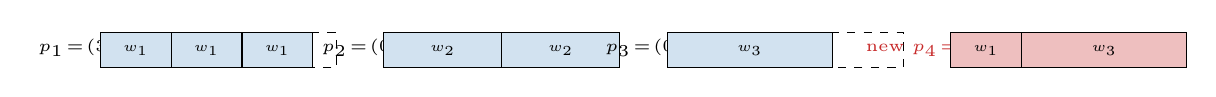
\begin{tikzpicture}[xscale=0.30,yscale=0.45,every node/.style={font=\tiny}]
    \begin{scope}[xshift=0cm]
      \node[above,scale=1.2]{$p_1\!=\!(3,0,0)$};
      \draw[fill=accent2!20] (0,0) rectangle (3,1);\node at (1.5,0.5){$w_1$};
      \draw[fill=accent2!20] (3,0) rectangle (6,1);\node at (4.5,0.5){$w_1$};
      \draw[fill=accent2!20] (6,0) rectangle (9,1);\node at (7.5,0.5){$w_1$};
      \draw[dashed] (9,0) rectangle (10,1);
    \end{scope}
    \begin{scope}[xshift=12cm]
      \node[above,scale=1.2]{$p_2\!=\!(0,2,0)$};
      \draw[fill=accent2!20] (0,0) rectangle (5,1);\node at (2.5,0.5){$w_2$};
      \draw[fill=accent2!20] (5,0) rectangle (10,1);\node at (7.5,0.5){$w_2$};
    \end{scope}
    \begin{scope}[xshift=24cm]
      \node[above,scale=1.2]{$p_3\!=\!(0,0,1)$};
      \draw[fill=accent2!20] (0,0) rectangle (7,1);\node at (3.5,0.5){$w_3$};
      \draw[dashed] (7,0) rectangle (10,1);
    \end{scope}
    \begin{scope}[xshift=36cm]
      \node[above,scale=1.2]{\textcolor{accent}{new $p_4\!=\!(1,0,1)$}};
      \draw[fill=accent!30] (0,0) rectangle (3,1);\node at (1.5,0.5){$w_1$};
      \draw[fill=accent!30] (3,0) rectangle (10,1);\node at (6.5,0.5){$w_3$};
    \end{scope}
  \end{tikzpicture}
  \end{center}
\begin{lstlisting}
master.addColumn(p1=(3,0,0), cost=1)             # covers item 1
master.addColumn(p2=(0,2,0), cost=1)             # covers item 2
master.addColumn(p3=(0,0,1), cost=1)             # covers item 3
pi = master.solve_dual()                         # ~ (1/3, 1/2, 1)
p_new = knapsack(profits=pi, weights=(3,5,7), W=10)   # -> (1,0,1)
master.addColumn(p_new, cost=1)                  # red. cost 1 - (1/3 + 1) < 0
\end{lstlisting}
  After a few iterations the LP settles at $z^{LP}=13.5$;
  $\lceil 13.5\rceil = 14$ is the IP optimum.
\end{frame}

\begin{frame}{Why no upper bound on $x_p$?}
  The LP we solve is
  \[
     \min \sum_p c_p\, x_p \quad
     \text{s.t.}\quad \sum_p a_{ip}\, x_p\;[\!=\!\text{or}\!\ge\!]\;b_i\;\;\forall i,\quad
     x_p \ge 0.
  \]
  We only declare $x_p\!\ge\!0$ -- \alert{never} an upper bound $x_p\!\le\!1$.

  \medskip
  \begin{itemize}\small
    \item The covering / partitioning constraint \alert{already bounds}
          $x_p$: in cutting stock $\sum_p x_p \le \sum_p a_{ip}\,x_p/a_{ip}$
          and in VRPTW $x_p\le \sum_p a_{ip}\,x_p = 1$ when the customer
          $i\in S_p$ exists. Bounds ``built in''.
    \item Adding $x_p\!\le\!1$ creates an extra dual $\mu_p\!\ge\!0$ on each
          column. The pricer would then need to compute
          $\redcost_p = c_p - \boldsymbol\pi\transpose\mathbf a_p + \mu_p$
          -- but $\mu_p$ depends on the column we're trying to find. That's
          a chicken-and-egg pricing problem.
    \item Dropping the upper bound also keeps the master sparse and lets
          simplex avoid degeneracy from artificial bound constraints.
  \end{itemize}
  \begin{keybox}[Rule]
    Continuous LP master: $x_p\!\ge\!0$, no upper bound. Integrality
    ($x_p\!\in\!\{0,1\}$) is only re-imposed inside heuristics or B\&P.
  \end{keybox}
\end{frame}

\begin{frame}{Initial columns -- bootstrap}
  $\rmp$ must be feasible from iteration 1. Two go-to recipes:
  \begin{itemize}\small
    \item \textbf{One column per covering constraint.} For VRPTW, one
          singleton route depot $\to i\to$ depot for each customer
          $i\in\mathcal N$ -- always feasible, gives a valid finite dual.
          For cutting stock, one ``one-item'' pattern per item type. This is
          what the lab does.
    \item \textbf{Slack / artificial variables.} Add a per-constraint slack
          $s_i\!\ge\!0$ with huge cost $M$ in the master objective. Always
          feasible regardless of the column pool. Drop slacks (or watch them
          drift to 0) as real columns enter.
  \end{itemize}
  \begin{keybox}[Rule of thumb]
    Either start with one route/pattern per customer/item, or add a slack
    column per constraint -- but \alert{never start empty}.
  \end{keybox}
  \begin{warnbox}[Why not start empty?]
    With an infeasible $\rmp$ the dual is unbounded: the pricer gets bogus
    prices and convergence is unreliable.
  \end{warnbox}
\end{frame}

\begin{frame}{Quick view -- Dantzig--Wolfe decomposition}
  Take any LP with block-diagonal structure
  \[
    \min c\transpose x \;\text{s.t.}\; A_0 x \ge b_0,\; x\in X = \{x:Bx\ge d,\,x\ge 0\}.
  \]
  $X$ a polyhedron $\Rightarrow$ every $x\in X$ writes as
  $x=\sum_p \lambda_p\, v_p + \sum_r \mu_r\, r_r$, $\lambda\in\Delta$, $\mu\ge 0$
  (vertices $v_p$, rays $r_r$). Substituting:
  \[
    \min \sum_p (c\transpose v_p)\lambda_p + \sum_r (c\transpose r_r)\mu_r
    \;\text{s.t.}\;
    \sum_p (A_0 v_p)\lambda_p+\sum_r (A_0 r_r)\mu_r\ge b_0,\;
    \mathbf 1\transpose\lambda=1.
  \]
  This is the \alert{master problem}; one variable per vertex/ray of $X$.
  Pricing = optimisation over $X$ with modified objective $c-\boldsymbol\pi A_0$.
\end{frame}

\begin{frame}{Why we are not deriving DW today}
  \begin{itemize}\small
    \item In our applications $X$ is implicit (set of routes, set of patterns)
          and we go straight to the path/pattern formulation -- no block
          structure to convexify on paper.
    \item DW gives the same master/pricing pair, with a clean formal status
          for the pricing oracle and the Lagrangian dual.
    \item Useful when you read the literature: Lagrangian relaxation of $A_0$,
          column generation and DW are all the same algorithm with different
          accents.
  \end{itemize}
  \vspace{0.5em}
  \begin{keybox}[One-line summary]
    Whether you start from ``the LP has too many columns'' (CG view) or
    from ``the LP has block structure that we want to push into a subproblem''
    (DW view), you get the same RMP--SP loop.
  \end{keybox}
\end{frame}

\begin{frame}{Geometric picture}
  \begin{columns}[T,onlytextwidth]
    \column{0.55\textwidth}
    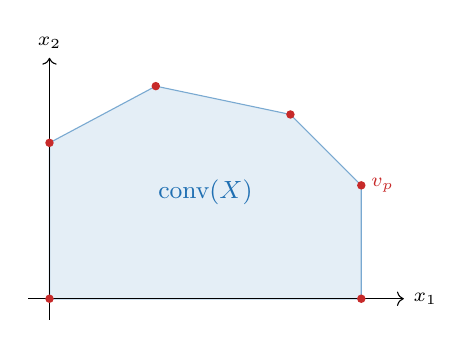
\begin{tikzpicture}[scale=0.9]
      \fill[accent2!12,draw=accent2!60] (0,0) -- (4.4,0) -- (4.4,1.6) -- (3.4,2.6) -- (1.5,3) -- (0,2.2) -- cycle;
      \node[accent2] at (2.2,1.5) {\small conv$(X)$};
      \draw[->] (-0.3,0) -- (5.0,0);
      \draw[->] (0,-0.3) -- (0,3.4);
      \foreach \p in {(0,0),(4.4,0),(4.4,1.6),(3.4,2.6),(1.5,3),(0,2.2)} {
        \fill[accent] \p circle (1.7pt);
      }
      \node[right, accent] at (4.4,1.6) {\scriptsize $v_p$};
      \node[right] at (5.0,0) {\scriptsize $x_1$};
      \node[above] at (0,3.4) {\scriptsize $x_2$};
    \end{tikzpicture}
    \column{0.45\textwidth}
    \small
    Each red dot is a feasible \emph{route} / \emph{pattern}. The master
    optimises a linear function on the convex hull of these dots, intersected
    with the linking constraints $A_0 x\ge b_0$.

    \medskip
    Pricing returns a vertex $v_p$ that improves the objective; it never
    enumerates the dots, it \alert{walks} on $X$ directly.
  \end{columns}
\end{frame}

\begin{frame}{Termination, in theory and in practice}
  \begin{itemize}\small
    \item There are finitely many extreme points in $X$, so CG terminates
          after finitely many iterations.
    \item In practice ``finitely'' can be \alert{thousands} of iterations on
          large instances.
    \item Last 5\% of iterations often produce columns that contribute almost
          nothing -- the famous \alert{tailing-off} effect (Part~4).
  \end{itemize}
  \vfill
  \begin{keybox}[Stopping criteria you'll see]
    \begin{itemize}\small
      \item Exact: pricer returns no negative-reduced-cost column.
      \item Heuristic: $\rmp$ improvement below threshold $\varepsilon$ for
            $K$ consecutive iterations.
      \item Bound-based: Lagrangian lower bound $\ge$ best known IP minus
            $\delta\%$.
    \end{itemize}
  \end{keybox}
\end{frame}

\begin{frame}{\textbf{[lab]} Exercise A -- Build the master in HiGHS}
  \begin{exbox}[Exercise A -- master \& initial columns]
    \begin{itemize}\small
      \item Open \texttt{lab/python/vrp/cg/master\_problem.py}.
      \item Implement \texttt{add\_constraints} (one $=\!1$ row per customer)
            and \texttt{set\_objective} (sum of route costs).
      \item In \texttt{vrp.py}, implement \texttt{generate\_initial\_paths}:
            one round-trip route per customer.
      \item Run \texttt{python -m vrp.tests.toy\_master} and check
            $z^{\rmp}_0$ matches the expected value printed in the test.
    \end{itemize}
    \alert{Time budget: 15 minutes.}
  \end{exbox}
\end{frame}

% =====================================================================
\section{Part 3 -- The pricing subproblem (RCSPP)}
% =====================================================================

\begin{frame}{What is RCSPP?}
  Given a digraph $G=(V,A)$ with arc costs $c_{uv}$ and \alert{resource}
  consumptions $\rho_{uv}^{(r)}$ for $r=1,\dots,R$, plus per-resource bounds
  $[\ell_v^{(r)},u_v^{(r)}]$ at each node:
  \[
     \min \sum_{(u,v)\in P} c_{uv} \quad
     \text{s.t.}\quad P\text{ is an } o\!\to\!d \text{ path with}\;
     \ell^{(r)}\le \mathcal R^{(r)}(P) \le u^{(r)}\;\forall r.
  \]
  $\mathcal R^{(r)}(P)$ = accumulated resource $r$ along $P$ (e.g.\ time, load).

  \medskip
  \begin{itemize}\small
    \item $R\!=\!0$ $\Rightarrow$ classical shortest path (Dijkstra/Bellman).
    \item Non-trivial resources $\Rightarrow$ NP-hard in general.
    \item In CG we have negative arc costs (because of duals), so we can't
          use Dijkstra naively even when there are no resources.
  \end{itemize}
\end{frame}

\begin{frame}{Resources, the workhorse abstraction}
  A \alert{resource} is any quantity that
  \begin{itemize}\small
    \item starts at some value at the origin,
    \item is updated along the path by an \alert{extension function}
          $f^{(r)}_{uv}\!:\R\!\to\!\R$,
    \item must satisfy a \alert{feasibility window} $[\ell^{(r)}_v,u^{(r)}_v]$ at every node $v$,
    \item supports a \alert{dominance relation} for label pruning.
  \end{itemize}

  \medskip
  Examples in VRPTW:
  \begin{tabular}{@{}llll@{}}
    \toprule
    Resource & Update & Window at $v$ & Dominance \\
    \midrule
    Distance / cost & $T'\!=\!T+c_{uv}$ & $(-\!\infty,+\!\infty)$ & $\le$ \\
    Time           & $T'\!=\!\max(T+s_u+t_{uv},a_v)$ & $[a_v,b_v]$ & $\le$ \\
    Load           & $Q'\!=\!Q+q_v$ & $[0,Q^{\max}]$ & $\le$ \\
    Visited set    & $S'\!=\!S\cup\{v\}$ & elementary, $v\notin S$ & $\subseteq$ \\
    \bottomrule
  \end{tabular}
  In our \texttt{rcspp} package these are encoded by the
  \texttt{ExtensionFunction}, \texttt{FeasibilityFunction},
  \texttt{DominanceFunction} triple.
\end{frame}

\begin{frame}{Label-setting algorithm (Desrochers \& Soumis, 1988)}
  A \alert{label} at node $v$ is a tuple
  $L=(v,\;\text{cost},\;\rho^{(1)},\dots,\rho^{(R)},\;\text{predecessor})$.

  \begin{algo}[Generic label-setting]
  \item Initialise: at origin $o$, push label $L_0$ with cost $0$ and resources at lower bounds.
  \item \textbf{while} unprocessed labels exist
  \item \Indent pick label $L$ at node $u$ (priority: cost or lex.\ on resources)
  \item \Indent \textbf{for} each arc $(u,v)\in A$
  \item \IndentTwo extend $L\to L'$ via $f_{uv}$
  \item \IndentTwo \textbf{if} $L'$ feasible \textbf{and} not dominated, store it
  \item \Indent dominate / discard newly dominated labels at $v$
  \item \textbf{end while}
  \item Best label at destination $d$ = optimal RCSPP path
  \end{algo}
  Correctness: dominance + monotone extensions $\Rightarrow$ no useful label
  is ever discarded.
\end{frame}

\begin{frame}{Dominance, the trick that keeps it tractable}
  \begin{tcolorbox}[colback=accent2!8,colframe=accent2!60,sharp corners,boxrule=0.4pt,
                    left=4pt,right=4pt,top=2pt,bottom=2pt]
  Label $L_1$ \alert{dominates} $L_2$ at the same node $v$ if
  \[
    \text{cost}(L_1)\le\text{cost}(L_2),\quad
    \rho^{(r)}(L_1)\le\rho^{(r)}(L_2)\;\;\forall r,
  \]
  with at least one strict inequality. Then any feasible completion of $L_2$
  is also feasible from $L_1$ and cheaper.
  \end{tcolorbox}

  \begin{itemize}\small
    \item Pruning power scales with the number of \alert{partially ordered}
          resources.
    \item Elementarity (set of visited customers) is \emph{not} totally
          ordered $\Rightarrow$ dominance is much weaker once we enforce it.
    \item Practical compromise: \alert{ng-routes} (Baldacci et al., 2011) --
          forbid revisits only inside small neighbourhoods $N_v$.
  \end{itemize}
\end{frame}

\begin{frame}{A worked RCSPP example}
  \begin{columns}[T,onlytextwidth]
    \column{0.58\textwidth}
    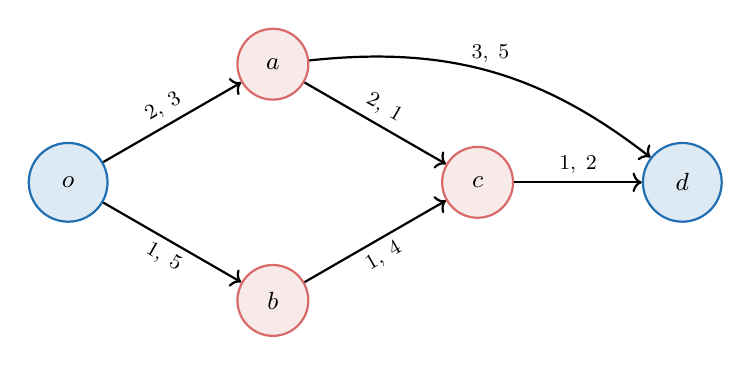
\begin{tikzpicture}[every node/.style={font=\small}]
      \tikzstyle{n} =[circle,draw,minimum size=9mm,inner sep=0pt,
                      fill=accent!10,draw=accent!70,thick];
      \tikzstyle{nd}=[circle,draw,minimum size=10mm,inner sep=0pt,
                      fill=accent2!15,draw=accent2,thick];
      \node[nd] (o) at (0,0) {$o$};
      \node[n]  (a) at (2.6,1.5) {$a$};
      \node[n]  (b) at (2.6,-1.5) {$b$};
      \node[n]  (c) at (5.2,0.0) {$c$};
      \node[nd] (d) at (7.8,0.0) {$d$};
      \draw[->,thick] (o) -- node[sloped,above,scale=0.85]{$2,\;3$} (a);
      \draw[->,thick] (o) -- node[sloped,below,scale=0.85]{$1,\;5$} (b);
      \draw[->,thick] (a) -- node[sloped,above,scale=0.85]{$2,\;1$} (c);
      \draw[->,thick] (b) -- node[sloped,below,scale=0.85]{$1,\;4$} (c);
      \draw[->,thick] (c) -- node[above,scale=0.85]{$1,\;2$} (d);
      \draw[->,thick] (a) to[bend left=22] node[above,scale=0.85]{$3,\;5$} (d);
    \end{tikzpicture}

    \medskip
    \scriptsize Each arc labelled $(c_{uv},\,\rho_{uv})$.\;
    Resource budget at $d$: $\rho(P)\le 7$.

    \column{0.39\textwidth}
    \scriptsize
    \begin{tabular}{@{}lcc@{}}
      \toprule
      Path & $\sum c$ & $\sum\rho$ \\
      \midrule
      $o\!\to\!a\!\to\!c\!\to\!d$ & $5$ & $6$ \cmark \\
      $o\!\to\!b\!\to\!c\!\to\!d$ & $3$ & $11$ \xmark \\
      $o\!\to\!a\!\to\!d$         & $5$ & $8$ \xmark \\
      \bottomrule
    \end{tabular}

    \medskip
    Optimum: $o\!\to\!a\!\to\!c\!\to\!d$, cost $5$.
  \end{columns}
  \medskip
  \alert{Shortest path and feasible path are not the same.} The cheaper
  $o\!\to\!b\!\to\!c\!\to\!d$ violates the resource budget.
\end{frame}

\begin{frame}{Elementary or not? coefficient $a_{ip}$ in the master}
  Two consistent ways to describe a route $p$ in the set-partitioning master:
  \begin{itemize}\small
    \item \textbf{Elementary}: every customer appears at most once,
          $a_{ip}\!=\!\mathbf 1[i\in S_p]\in\{0,1\}$. Coefficient is binary.
    \item \textbf{Non-elementary} (SPPRC): pricer may produce routes
          revisiting a customer; we set $a_{ip}\!=\!\#$ visits of $i$ in $p$,
          which can be $\ge 2$.
  \end{itemize}
  \begin{tcolorbox}[colback=accent!5,colframe=accent!60,sharp corners,boxrule=0.4pt]
    Both formulations are mathematically valid. The set-partitioning master
    enforces $\sum_p a_{ip} x_p = 1$ in either case; with $a_{ip}\!=\!2$
    for a route that visits $i$ twice, the LP simply needs to set $x_p\!=\!1/2$
    or pay heavily.
  \end{tcolorbox}
  \begin{itemize}\small
    \item Elementary: tighter LP, harder pricer (ESPPRC).
    \item Non-elementary: weaker LP (revisits allowed at LP level), much
          easier pricer (SPPRC).
    \item ng-routes interpolate: cheap pricer, almost-elementary LP.
  \end{itemize}
\end{frame}

\begin{frame}{ESPPRC vs SPPRC}
  \begin{tabular}{@{}p{0.40\textwidth}p{0.55\textwidth}@{}}
    \toprule
    \textbf{ESPPRC} & visit each node \alert{at most once}; pricing for
                      set-partitioning master with $=1$ constraints. \\
    \textbf{SPPRC}  & nodes may be revisited; pricing for
                      set-covering ($\ge 1$). \\
    \bottomrule
  \end{tabular}
  \medskip
  \begin{itemize}\small
    \item ESPPRC is \alert{strongly} NP-hard.
    \item SPPRC with non-negative reduced costs and \alert{integer}
          resources is solvable in pseudo-polynomial time.
    \item Most modern VRPTW solvers price ng-routes: between SPPRC and ESPPRC,
          they tighten dominance compared to SPPRC but stay tractable.
  \end{itemize}

  \begin{keybox}[Practical advice]
    Avoid solving the full \alert{ESPPRC} in general -- it explodes
    combinatorially. Start with \alert{SPPRC} pricing; if the master ends up
    with too many revisiting routes, switch to ng-routes. Reserve exact
    ESPPRC for small instances or for the last few branch-and-price nodes.
  \end{keybox}
\end{frame}

\begin{frame}{Heuristic vs exact pricing}
  \begin{tabular}{@{}lll@{}}
    \toprule
    Method & Cost per call & Returns \\
    \midrule
    Greedy / nearest-neighbour & $O(n^2)$ & 1 negative-cost route \\
    Heuristic label-setting & $O(n\cdot|A|)$ & a handful \\
    Exact label-setting (SPPRC / ESPPRC) & exp.\ in worst case & all neg.\ red.\ cost \\
    Bidirectional w.\ join & faster than fwd & same \\
    \bottomrule
  \end{tabular}
  \medskip
  \begin{itemize}\small
    \item During the first iterations, nobody calls the exact pricer.
    \item Hierarchy: greedy $\to$ ng-route $\to$ exact ESPPRC, escalate only when
          cheaper levels return $\redcost\ge 0$.
    \item For LP optimality, the \alert{last} pricing call must be exact.
    \item For the Lagrangian bound (Part 6), we also need a true lower bound
          from the pricer -- heuristic pricers are not enough.
  \end{itemize}
\end{frame}

\begin{frame}{Returning multiple columns per call}
  CG converges much faster if each pricing call adds many columns.

  \medskip
  \begin{itemize}\small
    \item Bidirectional / multi-label algorithms naturally produce many
          non-dominated sink labels with $\redcost<0$.
    \item Filter: keep only the $K$ best, or the most ``diverse'' (different
          customer subsets).
    \item Trade-off: more columns $\Rightarrow$ heavier $\rmp$.
    \item Typical $K\in\{20,50,100\}$ on Solomon-100.
  \end{itemize}
  \vfill
  \begin{tcolorbox}[colback=accent!5,colframe=accent!50,sharp corners,boxrule=0.4pt]
   In the lab, \texttt{VRP(K\_MAX=K)} caps the number of columns added per
   CG iteration. The \texttt{compare\_cg} runner sweeps $K$ for you.
  \end{tcolorbox}
\end{frame}

\begin{frame}[fragile]{The \texttt{rcspp} Python package, in 30 seconds}
\begin{lstlisting}
from rcspp.graph    import ResourceGraph
from rcspp._core.graph import Row
from rcspp.resource import (
    AdditionExtensionFunction,            # cost or load
    ValueDominanceFunction,               # <= dominance
    ValueCostFunction,
    TrivialFeasibilityFunction,           # no bound
    MinMaxFeasibilityFunction,            # [lo, hi]
    TimeWindowExtensionFunction,          # max(T+travel, a_v)
    TimeWindowFeasibilityFunction,        # T <= b_v
)
g = ResourceGraph()
g.add_real_resource(ext, feas, cost, dom)            # 1 call / resource
g.add_node(node_id, is_source, is_sink)
g.add_arc((dist, time, load),                        # base resource incr.
          o, d, arc_id, dist,                        # base cost = dist
          [Row(o, 1.0)])                             # 1*pi_o subtracted
g.update_reduced_costs(dual_by_id)                   # cheap re-pricing
solutions = g.solve()                                # Solution[]
\end{lstlisting}
  \begin{itemize}\small
    \item Each arc carries \alert{base costs} (no duals baked in) plus
          a list of dual \texttt{Row}s. The reduced cost is
          $\redcost_{uv}=c_{uv}^{\text{base}}-\sum_r \alpha_r\,\pi_{i_r}$.
    \item \alert{Build the graph once}; call
          \texttt{update\_reduced\_costs} every CG iteration -- no need
          to recreate nodes or arcs.
    \item \texttt{solve()} returns all sink labels with negative reduced
          cost, sorted ascending.
  \end{itemize}
\end{frame}

\begin{frame}{\textbf{[lab]} Exercise B -- Wire the pricing subproblem}
  \begin{exbox}[Exercise B -- arc costs \& RCSPP solve]
    \begin{itemize}\small
      \item In \texttt{vrp.py}, complete \texttt{add\_arc\_to\_graph}:
            arc cost $=d_{uv}-\pi_v$ (with $\pi_0:=0$), three resource
            increments (cost, time, demand), in the same order as the
            \texttt{add\_real\_resource} calls in
            \texttt{construct\_resource\_graph}.
      \item Replace the body of \texttt{solve\_subproblem} so that it
            constructs the resource graph with the latest duals and returns
            the result of \texttt{ResourceGraph.solve()}.
      \item Run \texttt{python -m vrp.tests.toy\_pricing} and check that the
            first negative-reduced-cost route on \texttt{toy.txt} matches
            the expected route printed by the test.
    \end{itemize}
    \alert{Time budget: 25 minutes.}
  \end{exbox}
\end{frame}

% =====================================================================
\section{Part 4 -- Making column generation fast}
% =====================================================================

\begin{frame}{Where the time goes}
  Profile of a typical CG iteration on VRPTW:
  \begin{center}
  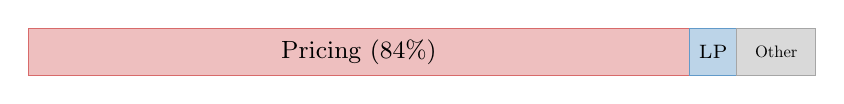
\begin{tikzpicture}
    \draw[fill=accent!30, draw=accent!70] (0,0) rectangle (8.4,0.6);
    \draw[fill=accent2!30, draw=accent2!70] (8.4,0) rectangle (9.0,0.6);
    \draw[fill=gray!30, draw=gray!70] (9.0,0) rectangle (10,0.6);
    \node at (4.2,0.3) {\small Pricing (84\%)};
    \node at (8.7,0.3) {\scriptsize\rotatebox{0}{LP}};
    \node[rotate=0,scale=0.6] at (9.5,0.3) {Other};
  \end{tikzpicture}
  \end{center}
  \begin{itemize}\small
    \item Rule of thumb: pricing is 70-95\% of total time.
    \item LP solve grows roughly linearly with the number of accumulated columns
          (warm-started simplex / interior point reuse).
    \item Memory: the column pool can balloon to millions of routes -- you
          will need a pruning strategy.
  \end{itemize}
\end{frame}

\begin{frame}{Trick 1 -- Multi-column pricing (revisited)}
  Add many columns per iteration to amortise the pricing.
  \begin{itemize}\small
    \item ``All non-dominated sink labels with $\redcost\!<\!-\varepsilon$''
    \item or top-$K$ by $\redcost$,
    \item or one column per ``corridor'' of the graph (diversity).
  \end{itemize}

  \medskip
  \textbf{Effect}: 5-30\% iteration count reduction, often 2x wall-clock.
  Not a strict free lunch -- on degenerate masters it can amplify cycling.
\end{frame}

\begin{frame}{Trick 2 -- Hierarchy of pricers}
  Inside the same path family, escalate cheap $\to$ expensive only when the
  cheap one finds no negative-reduced-cost column:
  \begin{center}
  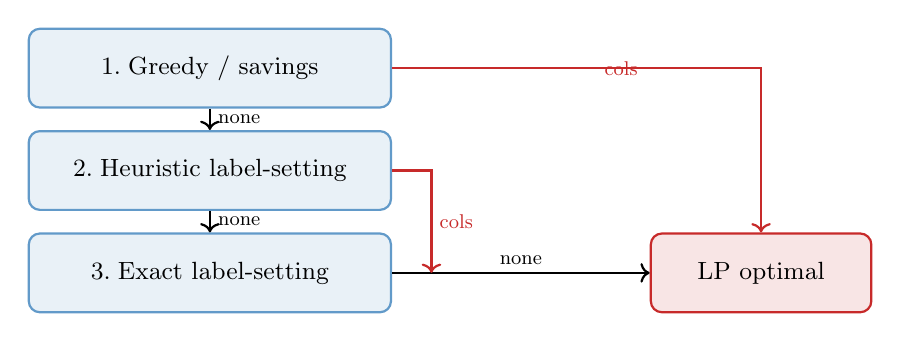
\begin{tikzpicture}[every node/.style={font=\small}]
    \tikzstyle{p}=[draw,rounded corners,minimum width=46mm,minimum height=10mm,
                   fill=accent2!10,draw=accent2!70,thick,align=center];
    \tikzstyle{stop}=[draw,rounded corners,minimum width=28mm,minimum height=10mm,
                   fill=accent!12,draw=accent,thick,align=center];
    \node[p]   (g)  at (0,2.6)  {1.\;Greedy / savings};
    \node[p]   (h)  at (0,1.3)  {2.\;Heuristic label-setting};
    \node[p]   (ex) at (0,0.0)  {3.\;Exact label-setting};
    \node[stop](sp) at (7.0,0.0){LP optimal};

    \draw[->,thick] (g.south)  -- node[right,scale=0.8]{none} (h.north);
    \draw[->,thick] (h.south)  -- node[right,scale=0.8]{none} (ex.north);
    \draw[->,thick] (ex.east)  -- node[above,scale=0.8]{none} (sp.west);

    \draw[->,thick,accent] (g.east)  -- ++(0.5,0) -| node[right,scale=0.8,pos=0.25]{cols} (sp.north);
    \draw[->,thick,accent] (h.east)  -- ++(0.5,0) -- node[right,scale=0.8]{cols} ++(0,-1.3);
  \end{tikzpicture}
  \end{center}
  \vspace{-0.3em}
  \begin{itemize}\small
    \item All three solve the \emph{same} pricing problem -- they differ only
          in how thoroughly they search.
    \item For LP optimality the \alert{last} call must be exact.
    \item The exact pricer is typically only used at the end of the root
          and at every B\&P node closure.
  \end{itemize}
\end{frame}

\begin{frame}{Path family is a separate choice}
  Don't confuse the algorithmic hierarchy above with the choice of
  \alert{path family}, which decides what counts as a feasible column:
  \begin{tabular}{@{}p{0.30\textwidth}p{0.62\textwidth}@{}}
    \toprule
    Family & Definition / pricing problem \\
    \midrule
    \textbf{SPPRC} & nodes can be revisited; coefficient $a_{ip}$ in master
                     can be $\ge 2$. Pseudo-poly with non-negative duals. \\
    \textbf{ng-routes} & nodes can be revisited only if the recently
                     visited set does not contain them. ``Almost
                     elementary'', partial dominance. \\
    \textbf{ESPPRC} & every customer visited at most once. Strongest LP,
                     pricer is strongly NP-hard. \\
    \bottomrule
  \end{tabular}
  \medskip
  \begin{itemize}\small
    \item These are not levels you escalate through during one CG run -- you
          \alert{pick one} (typically ng-routes) and stay with it.
    \item The only time you switch is to fix specific routes that visit
          customers more than once (Ryan-Foster, Part~6).
  \end{itemize}
\end{frame}

\begin{frame}{Trick 3 -- Stabilisation}
  Without stabilisation, dual prices oscillate wildly $\Rightarrow$ pricer
  produces useless or duplicate columns.

  \medskip
  Three popular schemes:
  \begin{itemize}\small
    \item \alert{Box-step / trust region}: bound the change in $\boldsymbol\pi$.
    \item \alert{Bundle / proximal}: quadratic penalty on
          $\|\boldsymbol\pi-\hat{\boldsymbol\pi}\|^2$.
    \item \alert{Dual-price smoothing} (Wentges):
          $\boldsymbol\pi^{(k+1)} = \alpha\,\boldsymbol\pi^{(k)} + (1-\alpha)\,
          \boldsymbol\pi^{(k)}_{\rmp}$ with $\alpha\in[0,1)$.
    \item \alert{Du Merle penalties}: artificial dual bounds via penalty
          variables in the master.
  \end{itemize}

  \medskip
  \begin{keybox}[Practical advice]
    Wentges smoothing is one extra line of code, makes a huge difference, and
    converges to the same optimum for $\alpha<1$. Start there.
  \end{keybox}
\end{frame}

\begin{frame}{Trick 4 -- Handling the column pool}
  \begin{itemize}\small
    \item Keep all columns generated; they will be needed at branching.
    \item Track each column's \alert{age} (= iters since last positive in $\rmp$).
    \item In the master LP, only \emph{warm-start} with active columns; pool
          stays on disk / in a side structure.
    \item At a branching decision, only columns \emph{compatible} with the
          branch are passed on (filter by Ryan-Foster or arc-branch criterion).
  \end{itemize}
\end{frame}

\begin{frame}{Trick 5 -- Fast LP re-optimisation}
  \begin{itemize}\small
    \item Adding columns is a \alert{trivial} re-optimisation: simplex stays
          dual feasible, primal-feasible after a few pivots.
    \item Use the \alert{primal simplex} after a column add (fewer pivots
          than dual).
    \item Conversely, after \alert{adding a constraint or branching},
          dual simplex is the right re-optimisation.
    \item HiGHS, Clp, Gurobi all expose explicit ``add column'' APIs --
          avoid rebuilding the model.
  \end{itemize}
  \medskip
  \begin{warnbox}[Beware]
    Building the LP from scratch each iteration (as in our didactic code)
    is fine for a workshop, terrible for production. After this morning, the
    first thing you'll change is to keep the LP alive across iterations.
  \end{warnbox}
\end{frame}

\begin{frame}{Trick 6 -- Tailing-off and early termination}
  \begin{columns}[T,onlytextwidth]
    \column{0.55\textwidth}
    \centering
    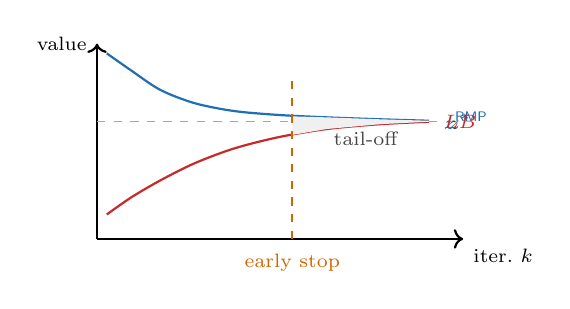
\begin{tikzpicture}[scale=0.62,every node/.style={font=\scriptsize}]
      % axes
      \draw[->,thick] (0,0) -- (7.5,0) node[below right]{iter.\ $k$};
      \draw[->,thick] (0,0) -- (0,4.0) node[left]{value};
      % horizontal optimum
      \draw[dashed,gray!70] (0,2.4) -- (7.0,2.4);
      \node[gray!50!black,right] at (7.0,2.4) {$z^*$};
      % z^RMP curve
      \draw[thick,accent2] plot[smooth] coordinates {
        (0.2,3.8) (0.7,3.45) (1.3,3.05) (2.0,2.78) (2.8,2.62)
        (3.7,2.54) (4.7,2.49) (5.8,2.45) (6.8,2.42)};
      \node[accent2,right] at (6.9,2.42) {$z^{\rmp}$};
      % LB curve
      \draw[thick,accent] plot[smooth] coordinates {
        (0.2,0.5) (0.7,0.85) (1.3,1.20) (2.0,1.55) (2.8,1.85)
        (3.7,2.08) (4.7,2.25) (5.8,2.35) (6.8,2.40)};
      \node[accent,right] at (6.9,2.39) {$LB$};
      % tail shading
      \fill[gray!12]
        (4.0,2.51) -- (4.7,2.49) -- (5.8,2.45) -- (6.8,2.42) --
        (6.8,2.40) -- (5.8,2.35) -- (4.7,2.25) -- (4.0,2.13) -- cycle;
      \node[gray!55!black] at (5.5,2.05) {tail-off};
      % early-stop line
      \draw[dashed,thick,orange!80!black] (4.0,0) -- (4.0,3.4);
      \node[orange!80!black,below=2pt] at (4.0,0) {early stop};
    \end{tikzpicture}
    \column{0.42\textwidth}
    \small
    \begin{itemize}\setlength{\itemsep}{4pt}
      \item $z^{\rmp}$ decreases very slowly at the end (\alert{tailing-off}).
      \item The Lagrangian bound $LB$ (Trick~7) only catches up on the
            last few iterations.
    \end{itemize}
    \medskip
    \textbf{Early stop when}
    \begin{itemize}\setlength{\itemsep}{2pt}
      \item rel.\ LP improvement $<\varepsilon$ for $K$ iters,
      \item $LB$ stagnates within tolerance, or
      \item time / iteration budget exhausted.
    \end{itemize}
    Stopping early kills $z^{\rmp}$ as a bound; $LB$ stays valid.
  \end{columns}
\end{frame}

\begin{frame}{\textbf{[ask the room]} How do we bound the LP early?}
  At iteration $k$, the master value $z^{\rmp_k}$ is an \alert{upper}
  bound on the LP -- it can only decrease as we add columns.
  \medskip
  \begin{keybox}[Question]
    \begin{itemize}
      \item How do we get a \alert{lower} bound on $z^*$ \emph{before} CG
            converges?
      \item What information do we already have at iteration $k$?
            (Hint: we just solved the pricing optimum exactly.)
    \end{itemize}
  \end{keybox}
  \medskip
  \emph{Answer on the next slide -- it's the Lagrangian bound.}
\end{frame}

\begin{frame}{Trick 7 -- The Lagrangian lower bound}
  At any CG iteration with current dual $\boldsymbol\pi$ and exact pricing
  optimum
  $\redcost^{*} = \min_{p\in\mathcal P}\,c_p-\boldsymbol\pi^{\!\top}\!\mathbf a_p$,
  \[
    z^* \;\ge\; \boldsymbol\pi^{\!\top}b
                \;+\; K\cdot \min(0,\,\redcost^{*})
        \;=:\;\text{LB}(\boldsymbol\pi),
  \]
  where $K$ is the number of vehicles and $b$ is the master RHS vector.
  \begin{itemize}\small
    \item For VRPTW with $b_i\!=\!1$: $LB = \sum_{i\in\mathcal N}\pi_i + K\,\redcost^{*}$.
    \item Valid \alert{at every iteration}, unlike $z^{\rmp}$ which is a true bound only at LP convergence.
    \item This requires the master to include the
          \alert{vehicle-count constraint} $\sum_p x_p\le K$ -- without it,
          the Lagrangian relaxation is unbounded below.
    \item Heuristic pricers do \alert{not} give a valid LB; only the exact
          pricer does.
  \end{itemize}
\end{frame}

\begin{frame}[fragile]{The bound in 4 lines of Python}
\begin{lstlisting}
def lagrangian_bound(mp_dual_by_id, sigma, pricing_sols, K):
    """LB = sum(pi_i) + K*sigma + K*min(0, min_redcost)."""
    pi_sum = sum(mp_dual_by_id.values())
    redc   = min((s.cost for s in pricing_sols), default=0.0)
    return pi_sum + K * sigma + K * min(0.0, redc)
\end{lstlisting}
  \begin{itemize}\small
    \item \texttt{sigma} is the dual on the vehicle-count constraint.
    \item Print this every iteration: it must increase (with smoothing)
          and end equal to $z^{\rmp}$ at LP optimum.
    \item Use it as the \alert{stop rule} at the root and as the
          \alert{prune rule} in B\&P.
  \end{itemize}
\end{frame}

\begin{frame}{Two new ways to stop CG early (lab \texttt{gap\_pct} \& \texttt{incumbent\_ub})}
  In the lab, \texttt{VRP.solve\_cg(incumbent\_ub, gap\_pct)} can stop
  before pricing returns $\redcost^*\ge 0$:
  \begin{itemize}\small
    \item \textbf{UB cut} -- when $LB\ge UB-\varepsilon$, the
          subtree is already proved optimal: no point in adding more columns.
          B\&P passes the current incumbent down to each child's CG run.
    \item \textbf{Gap cut} -- when $(z^{\rmp}-LB)/|z^{\rmp}|\le\delta\%$.
          Useful at the root for an approximate $\delta$-optimal LP.
  \end{itemize}
  \begin{keybox}[Why a gap stop is acceptable]
    A solver run with \texttt{gap\_pct=2} returns $z^{\rmp}$ and an LB
    that bracket $z^*$ within $2\%$ -- still a certified bound, even if
    incomplete. Often saves the last 80\% of iterations spent in
    tailing-off.
  \end{keybox}
\end{frame}

\begin{frame}{Trick 8 -- Symmetry and elementarity}
  \begin{itemize}\small
    \item In identical-vehicle VRP, set-partitioning is naturally
          \alert{symmetry-free} (one variable per route, regardless of vehicle).
    \item Cutting stock: identical rolls disappear in pattern formulation.
    \item Watch out for accidentally symmetric objectives: if your route cost
          $c_p$ does not depend on which vehicle uses it, drop vehicle indices
          everywhere.
    \item Elementarity vs SPPRC: revisits are LP-feasible only when the dual
          variables of revisited customers are positive enough to make the
          loop ``profitable''. ng-routes give you 90\% of elementarity for
          10\% of the work.
  \end{itemize}
\end{frame}

\begin{frame}{Putting it all together (efficient CG loop)}
\begin{algo}[Efficient column generation]
\item paths $\leftarrow$ initial columns (heuristic)
\item LP $\leftarrow$ build $\rmp$ on \texttt{paths}
\item iter $\leftarrow$ 0
\item \textbf{repeat}
\item \Indent solve LP $\Rightarrow$ duals $\pi$
\item \Indent $\pi \leftarrow$ smooth($\pi^{prev}$, $\pi$) \quad\textcolor{accent2}{\# Wentges}
\item \Indent $S \leftarrow$ greedy\_pricer($\pi$);
\item \IndentTwo \textbf{if} $S=\varnothing$: $S\leftarrow$ ng\_pricer
\item \IndentTwo \textbf{if} $S=\varnothing$: $S\leftarrow$ exact
\item \Indent \textbf{if} $S=\varnothing$: \textbf{break}
\item \Indent keep top-$K$ columns from $S$, add to LP (warm start)
\item \Indent compute LB; \textbf{if} $z^{\rmp}-\text{LB}\le\delta$: \textbf{break}
\item \textbf{end repeat}
\end{algo}
\end{frame}

\begin{frame}{\textbf{[lab]} Exercise C -- multi-column, smoothing, LB}
  \begin{exbox}[Exercise C -- efficient CG]
    \begin{itemize}\small
      \item Cap the number of columns added per iteration with the parameter
            \texttt{K\_MAX}; try $K\!\in\!\{1,5,20,100\}$ on
            \texttt{R101\_25.txt} and record total iterations \& wall-clock.
      \item Wentges smoothing: $\boldsymbol\pi\!\leftarrow\!
            \alpha\boldsymbol\pi^{prev}\!+\!(1-\alpha)\boldsymbol\pi$,
            $\alpha\!\in\![0.3,0.7]$.
      \item Implement
            \texttt{lagrangian\_bound(\dots)} (Trick 7) and print it every
            iteration. Stop CG when $z^{\rmp}\!-\!LB\le\delta$.
      \item \alert{Don't rebuild the master from scratch}: each CG iteration
            just calls \texttt{master.add\_column(\dots)} on the new
            columns, then re-solves the LP (warm-started simplex).
    \end{itemize}
    \alert{Time budget: 25 minutes.}
  \end{exbox}
  \begin{keybox}[Why we don't rebuild]
    Adding a column is a primal-feasible perturbation: simplex needs
    only a handful of pivots. Rebuilding from scratch throws the basis
    away and is the single biggest performance hit we'll see.
  \end{keybox}
\end{frame}

% =====================================================================
\section{Part 5 -- From LP to integer (heuristics)}
% =====================================================================

\begin{frame}{The LP is solved -- now what?}
  \begin{itemize}\small
    \item Solving the LP relaxation of the master gives a fractional
          $\bar x\in[0,1]^{|\widetilde{\mathcal P}|}$.
    \item Even if $\bar x$ is integer feasible, that is rare in real instances.
    \item Two families of next steps:
    \begin{itemize}\small
      \item \alert{Heuristic}: get a good integer solution fast, no
            optimality guarantee.
      \item \alert{Exact}: branch-and-price (Part 6).
    \end{itemize}
    \item Today we will use both: heuristics give a working incumbent in
          the lab, and we will then plug it into a small \alert{branch-and-price}
          loop (Part~6 + Exercise~E) that closes the optimality gap with the
          Lagrangian bound.
  \end{itemize}
\end{frame}

\begin{frame}{Heuristic 1 -- Restricted Master Heuristic (RMH)}
  Once CG terminates at the root, freeze the column pool $\widetilde{\mathcal P}$
  and solve
  \[
     z^{\text{RMH}} \;=\; \min \sum_{p\in\widetilde{\mathcal P}} c_p\, x_p
     \;\;\text{s.t.}\;\; A\, x \ge b,\;\; x_p\in\{0,1\}.
  \]
  \begin{itemize}\small
    \item Just hand the pool to a MIP solver (HiGHS, CBC, Gurobi).
    \item Quality depends entirely on the column diversity in the pool.
    \item Fast on small/medium VRP, often within 1-2\% of optimal on Solomon-25.
    \item Will be the \alert{first integer solver} we plug in the lab.
  \end{itemize}
  \vfill
  \begin{warnbox}[Caveat]
    The pool is generated for \emph{LP} optimality, not for integrality.
    On hard instances RMH can be feasibility-infeasible -- solve a
    set-covering relaxation as a fallback.
  \end{warnbox}
\end{frame}

\begin{frame}{Heuristic 2 -- Diving (price-and-fix)}
  Branch-and-bound with no backtrack and no bound checks.

  \medskip
  \begin{algo}[Diving heuristic]
  \item solve root CG; let $\bar x$ be its LP solution
  \item \textbf{repeat}
  \item \Indent pick column $p^*$ with $\bar x_{p^*}$ closest to 1 (or largest)
  \item \Indent fix $x_{p^*}\!=\!1$
  \item \Indent re-run CG on the residual master (warm-started)
  \item \Indent re-solve LP $\Rightarrow$ new $\bar x$
  \item \textbf{until} master integer (or infeasible)
  \end{algo}
  \begin{itemize}\small
    \item Each fix shrinks the residual problem (covered customers are
          locked).
    \item Convergence is fast: at most $|\mathcal N|$ fixes.
    \item Often beats RMH because it drives \alert{new compatible columns}
          at each fix.
  \end{itemize}
\end{frame}

\begin{frame}{Diving variants}
  \begin{itemize}\small
    \item \textbf{Multi-fix diving.} Fix several columns at once each
          iteration -- faster, lower quality.
    \item \textbf{LP-rounding dive.} Round $\bar x$ aggressively then resolve
          LP; cheap warm-start.
    \item \textbf{Limited-discrepancy diving (LDS).} Allow at most $K$
          ``mistakes'' along the dive -- a mistake is a fix that disagrees
          with the LP recommendation (e.g.\ second-best column instead of
          the closest-to-1). Equivalent to a depth-first search bounded by
          discrepancy budget $K$. Catches situations where the LP advice was
          wrong on one or two early fixes; keeps the runtime essentially
          linear in $K$.
    \item \textbf{Restart diving.} Re-run dive from new random seeds; pick best.
  \end{itemize}

  \medskip
  \begin{keybox}[For the lab]
    Implement plain diving first: pick column with largest $\bar x_p$, fix to
    1, re-run CG. 30 lines.
  \end{keybox}
\end{frame}

\begin{frame}{Heuristic 3 -- Price-and-branch (no bounding)}
  \begin{itemize}\small
    \item Run B\&P but \alert{do not prune by bound}: keep only the
          \alert{feasibility} cuts (drop branches that the master proves
          infeasible). The Lagrangian / LP bound is computed but not used
          for pruning.
    \item Effect: the search becomes a heuristic ``deep tree'' that follows
          fractional structure but never gives up on a node because of bound.
    \item Combined with depth-first search and a good incumbent heuristic
          (RMH at every node), this finds high-quality integer solutions
          quickly without exploring the whole tree.
    \item Often used as the warm-start of the exact B\&P -- the incumbent
          it produces tightens pruning later.
  \end{itemize}

  \medskip
  Hierarchy of heuristics in a serious solver:
  \[
    \text{RMH} \;\longrightarrow\; \text{LP-rounding}
                  \;\longrightarrow\; \text{plain diving}
                  \;\longrightarrow\; \text{LDS dive}
                  \;\longrightarrow\; \text{full B\&P}.
  \]
\end{frame}

\begin{frame}{When the heuristic is enough}
  \begin{itemize}\small
    \item Operational use cases (daily routing): a 1-2\% gap heuristic, run
          inside a refresh budget of a few minutes, is usually preferable to
          an overnight optimum.
    \item Tactical / strategic studies (yearly fleet design): you want the
          true optimum -- branch-and-price.
    \item \textbf{Sensitivity analyses.} If you need the marginal value of
          servicing customer $i$ (e.g.\ to decide whether to insert a new
          order, to negotiate price, or to compute opportunity costs across
          scenarios), you read it off the master dual $\pi_i$. Heuristic
          dives produce duals coming from intermediate restricted masters --
          they are \alert{not} the true LP duals of the original problem
          and can shift by 30--50\% between two consecutive dives. For
          reliable parametric output:
          \begin{itemize}\scriptsize
            \item solve the root CG to LP optimality, take its duals
                  (\emph{RMH at root only}), or
            \item run full B\&P and read duals at the optimal node.
          \end{itemize}
          Anything in between is fine for an objective value but unsafe for
          marginal-cost reasoning.
  \end{itemize}
\end{frame}

\begin{frame}{\textbf{[lab]} Exercise D -- Heuristic IP on the column pool}
  \begin{exbox}[Exercise D -- RMH then plain dive]
    \begin{itemize}\small
      \item After CG converges at the root, take the column pool and call
            \texttt{MasterProblem.solve(relax=False)}: that's the
            Restricted-Master Heuristic. Record incumbent value.
      \item Implement plain diving: pick the column $p^*$ with largest
            $\bar x_{p^*}$, set its upper bound to $1$ in the master, re-run
            CG, repeat until integer or infeasible.
      \item Compare RMH vs.\ diving on \texttt{R101\_25.txt} -- which gives
            the better incumbent? Which is faster?
    \end{itemize}
    \alert{Time budget: 25 minutes.}
  \end{exbox}
\end{frame}

% =====================================================================
\section{Part 6 -- Branch-and-Price}
% =====================================================================

\begin{frame}{Branch-and-price in one sentence}
  \begin{tcolorbox}[colback=accent!8,colframe=accent,sharp corners,boxrule=0.6pt]
  \textbf{Branch-and-bound on the master IP, where every node's LP relaxation
  is solved by column generation.}
  \end{tcolorbox}

  \medskip
  Three things change between B\&B and B\&P:
  \begin{enumerate}\small
    \item The LP at each node is huge $\Rightarrow$ solve it by CG.
    \item Branching on a master variable $x_p$ destroys the pricing structure
          $\Rightarrow$ branch \alert{on something else}.
    \item Every node needs valid columns; the column pool must be filtered to
          remain compatible with the branch.
  \end{enumerate}
\end{frame}

\begin{frame}{The naive branch (don't do this)}
  Just branching on a fractional master variable
  \[
     x_p = 0.5 \;\Longrightarrow\; \text{down: } x_p\le 0,\quad
                                   \text{up: } x_p\ge 1.
  \]
  \begin{itemize}\small
    \item Up-branch: fine -- $x_p\!\ge\!1$ locks column $p$ in the
          incumbent; the residual master is solved by CG with the locked
          column counted in the constraint slack.
    \item Down-branch: \alert{forbid one specific column} $p$. The pricer
          needs to enumerate ``all paths except $p$'' -- equivalent to a
          combinatorial $k$-shortest-path problem, which is much harder than
          plain SPPRC and \alert{breaks dominance}.
    \item The tree is also extremely unbalanced (one excluded column among
          $10^{20}$).
  \end{itemize}
  \begin{warnbox}[Take-away]
    Never branch on the master variables themselves.
  \end{warnbox}
\end{frame}

\begin{frame}{\textbf{[ask the room]} How would you branch?}
  Imagine the LP returns
  $\bar x_{p_1}=0.5$, $\bar x_{p_2}=0.5$, $\bar x_{p_3}=0$, …
  with $p_1$ and $p_2$ visiting partly different customers.

  \medskip
  \begin{keybox}[Question]
    \begin{itemize}
      \item Why does \alert{$x_p\!\le\!0$ vs $x_p\!\ge\!1$} (branching on the
            master variable) destroy the pricer?
      \item Find a binary criterion on \emph{customer pairs} that always
            shows fractionality whenever $\bar x$ is fractional.
    \end{itemize}
  \end{keybox}
  \medskip
  \emph{The answer is the Ryan-Foster rule -- next slide.}
\end{frame}

\begin{frame}{Ryan-Foster branching (set-partitioning case)}
  Set-partitioning constraints $\sum_p a_{ip}\,x_p = 1$. If $\bar x$ is fractional,
  there must exist customers $i,j$ such that
  \[
    \sum_{p:\,i,j\in S_p} \bar x_p \;\in\; (0,1),
  \]
  i.e.\ $i$ and $j$ are \alert{sometimes} together, \alert{sometimes} not.

  \medskip
  Two-way branch:
  \begin{itemize}\small
    \item \textbf{Together}: keep only routes that visit \alert{both or neither}.
          Implement by \emph{merging} $i$ and $j$ into a single node with
          combined demand and the time window
          $[a_i,b_i]\cup[a_j,b_j]$ (the union of the windows).
    \item \textbf{Apart}: forbid routes that visit \alert{both}. Implement by
          deleting all $i\!\to\!\dots\!\to\!j$ paths from the pricing graph.
  \end{itemize}
  Pricing structure is preserved on both branches.
\end{frame}

\begin{frame}{Ryan-Foster, the picture}
  Top: original pricing graph.\;Bottom-left: \emph{together}-branch.\;
  Bottom-right: \emph{apart}-branch.
  \begin{center}
  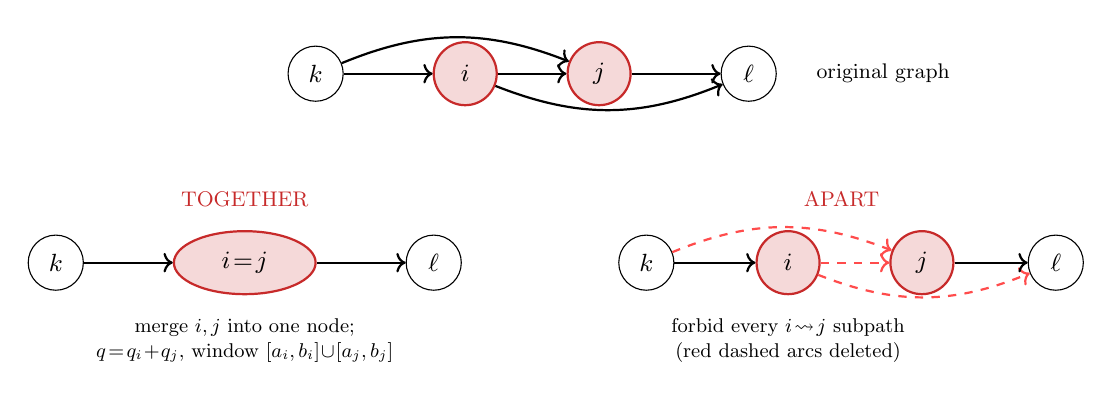
\begin{tikzpicture}[every node/.style={font=\small}]
    \tikzstyle{c}=[circle,draw,minimum size=7mm,inner sep=0pt,fill=white];
    \tikzstyle{ij}=[circle,draw,minimum size=8mm,inner sep=0pt,fill=accent!18,draw=accent,thick];
    \tikzstyle{merged}=[ellipse,draw,minimum width=18mm,minimum height=8mm,
                        fill=accent!18,draw=accent,thick,inner sep=0pt];
    % --- top: original ---
    \begin{scope}[yshift=2.0cm]
      \node[c]  (k0)  at (-2.5,0)  {$k$};
      \node[ij] (i0)  at (-0.6,0)  {$i$};
      \node[ij] (j0)  at ( 1.1,0)  {$j$};
      \node[c]  (l0)  at ( 3.0,0)  {$\ell$};
      \draw[->,thick] (k0)--(i0); \draw[->,thick] (i0)--(j0); \draw[->,thick] (j0)--(l0);
      \draw[->,thick] (k0) to[bend left=22]  (j0);
      \draw[->,thick] (i0) to[bend right=22] (l0);
      \node[right=4mm of l0,scale=0.85]{original graph};
    \end{scope}
    % --- bottom-left: together ---
    \begin{scope}[xshift=-3.4cm,yshift=-0.4cm]
      \node[c]      (k1)  at (-2.4,0)  {$k$};
      \node[merged] (ij1) at ( 0.0,0)  {$i\!=\!j$};
      \node[c]      (l1)  at ( 2.4,0)  {$\ell$};
      \draw[->,thick] (k1)--(ij1); \draw[->,thick] (ij1)--(l1);
      \node[below=2mm of ij1,scale=0.8,align=center]
       {merge $i,j$ into one node;\\$q\!=\!q_i\!+\!q_j$, window $[a_i,b_i]\!\cup\![a_j,b_j]$};
      \node[above=2mm of ij1,accent,scale=0.85]{TOGETHER};
    \end{scope}
    % --- bottom-right: apart ---
    \begin{scope}[xshift=4.1cm,yshift=-0.4cm]
      \node[c]  (k2)  at (-2.4,0)  {$k$};
      \node[ij] (i2)  at (-0.6,0)  {$i$};
      \node[ij] (j2)  at ( 1.1,0)  {$j$};
      \node[c]  (l2)  at ( 2.8,0)  {$\ell$};
      \draw[->,thick] (k2)--(i2);
      \draw[->,red!70,dashed,thick] (i2)--(j2);
      \draw[->,red!70,dashed,thick] (i2) to[bend right=22] (l2);
      \draw[->,red!70,dashed,thick] (k2) to[bend left=22]  (j2);
      \draw[->,thick] (j2)--(l2);
      \node[below=2mm of i2,scale=0.8,align=center]
       {forbid every $i\!\rightsquigarrow\!j$ subpath\\(red dashed arcs deleted)};
      \node[above=2mm of i2,accent,scale=0.85,xshift=8mm]{APART};
    \end{scope}
  \end{tikzpicture}
  \end{center}
  \vspace{-0.2em}
  \begin{keybox}[Key property]
    Both branches modify only the pricing \alert{graph}; the pricer code,
    dominance and resources are unchanged.
  \end{keybox}
\end{frame}

\begin{frame}{Branching on arcs / flow}
  Define the \alert{aggregated arc flow}
  \[
    y_{uv} \;=\; \sum_{p\,:\,(u,v)\in p} x_p .
  \]
  If $\bar y_{uv}\in(0,1)$, branch on $y_{uv}\le 0$ vs $y_{uv}\ge 1$.

  \medskip
  \begin{itemize}\small
    \item Down-branch: \alert{remove arc $(u,v)$} from pricing graph.
    \item Up-branch: \alert{force arc $(u,v)$} -- contract endpoints into a
          single super-node with merged time window.
    \item Universally compatible with VRP, scheduling, network design.
    \item Often produces more balanced trees than Ryan-Foster.
  \end{itemize}
\end{frame}

\begin{frame}{Branching on resources / time / load}
  When neither Ryan-Foster nor arc branching gives fractionality, branch on a
  resource:
  \[
     \tau_v \;=\; \sum_p\, t_v(p)\, \bar x_p \quad
     \text{(expected start time at } v\text{)}.
  \]
  Branch $\tau_v\le \lfloor\bar\tau_v\rfloor$ vs $\tau_v\ge \lceil\bar\tau_v\rceil$.

  \begin{itemize}\small
    \item Implemented by \alert{splitting the time window} of $v$ into two
          halves between branches.
    \item Same trick for vehicle load, working hours, etc.
    \item Useful late in the tree when only a few customers remain
          fractional.
  \end{itemize}

  \begin{keybox}[Modern recipe]
    Combine: arc branching first, Ryan-Foster on tied customers, resource
    branching for the remainder. All three preserve pricing structure.
  \end{keybox}
\end{frame}

\begin{frame}{The Lagrangian bound (Lasdon, 1970; Vanderbeck, 2006)}
  Master LP value $z^{\rmp}$ is \alert{not} a valid lower bound until CG converges.
  The Lagrangian bound is a valid lower bound at \alert{every} CG iteration.

  \medskip
  Let $\boldsymbol\pi$ be the current dual and let
  $\redcost^* = \min_{p\in\mathcal P}\, c_p - \boldsymbol\pi\transpose \mathbf a_p$
  be the pricing optimum. Then for the master MP with convexity (one
  vehicle/object):
  \[
    z^* \;\ge\; \boldsymbol\pi\transpose b \;+\; \redcost^*\quad
    \text{(Lagrangian dual at } \boldsymbol\pi\text{).}
  \]
  For multi-vehicle / multi-roll, with $K$ identical resources:
  \[
    z^* \;\ge\; \boldsymbol\pi\transpose b \;+\; K\cdot \redcost^*.
  \]
  Combine with the master LP: $z^* \le z^{\rmp}$, but at any time
  $z^*\ge\boldsymbol\pi\transpose b + K\redcost^*$.
\end{frame}

\begin{frame}{Why the Lagrangian bound matters}
  \begin{itemize}\small
    \item It \alert{monotonically increases} (with the right post-processing)
          and gives a valid stopping rule before LP convergence.
    \item Plug it into B\&P node pruning -- close branches whose Lagrangian
          bound exceeds the incumbent before paying for full LP convergence.
    \item Required ingredient for the \alert{integrated} dual stabilisation
          + bound machinery in modern solvers (BaPCod, VRPSolver, GCG).
    \item In our lab, you'll print it every iteration and watch it close in
          on the LP.
  \end{itemize}
  \vfill
  \begin{warnbox}[Subtle point]
    The bound uses $K\cdot\redcost^*$ \emph{only} if the pricer's
    $\redcost^*$ is a \alert{true} minimum -- heuristic pricers don't give a
    valid bound.
  \end{warnbox}
\end{frame}

\begin{frame}{The B\&P algorithm template}
\begin{algo}[Branch-and-price]
\item $\text{UB}\leftarrow +\infty$;\;\; open $\leftarrow\{$root$\}$;\;\; global\_LB $\leftarrow -\infty$
\item \textbf{while} open non-empty
\item \Indent $N \leftarrow$ pick-next(open) \quad\textcolor{accent2}{\# best-first OR depth-first dive}
\item \Indent \textbf{if} $N.\text{LB}\ge\text{UB}-\varepsilon$: \textbf{prune}
\item \Indent run CG on $N$ \emph{passing} UB;\; \quad\textcolor{accent2}{\# CG stops early if $LB\ge UB$}
\item \Indent global\_LB $\leftarrow \min(N.\text{LB},\;\min_{M\in\text{open}} M.\text{LB})$
\item \Indent \textbf{if} $(\text{UB}-\text{global\_LB})/|\text{UB}|\le\delta\%$: \textbf{stop} (gap reached)
\item \Indent \textbf{if} $N.\text{LB}\ge\text{UB}-\varepsilon$: \textbf{prune}
\item \Indent \textbf{if} LP integer: $\text{UB}\leftarrow\min(\text{UB},\,z^{\rmp})$; \textbf{prune}
\item \Indent \textbf{else} run heuristic (dive at root, RMH every $X$); update UB
\item \Indent pick branching arc $(u,v)$; create down, up children
\item \Indent \textbf{if} depth\_first: process \emph{up}-child immediately; queue down
\item \Indent \textbf{else}: queue both, sort open by LB
\item \textbf{end while}
\end{algo}
  \begin{itemize}\small
    \item \alert{Depth-first} (default in the lab): dive into the up-child --
          tighter constraints, fewer feasible columns, often integer fast.
    \item \alert{Best-first}: explore the open node with the smallest LB --
          best LB growth but heavier memory.
    \item \alert{global\_LB} is the smallest LB across \emph{all} open
          nodes; pair it with UB to certify a gap.
  \end{itemize}
\end{frame}

\begin{frame}{Cut-and-price -- one sentence}
  Add valid inequalities (subset-row, capacity, clique\dots) to the master.
  Each cut introduces a dual variable that the pricer must include in the
  reduced cost. Most modern solvers (BaPCod, VRPSolver, GCG, RouteOpt) do
  this, with the so-called \alert{subset-row cuts} being particularly potent
  for VRPTW. Out of scope today -- see
  Desrosiers, L\"ubbecke, Desaulniers \& Gauthier (2026), the open-access
  book in your folder (ISBN 978-3-031-96917-1), and Pecin et al.\ (2017) for
  the canonical SR-cut treatment.
\end{frame}

\begin{frame}{Putting all of B\&P on one slide}
  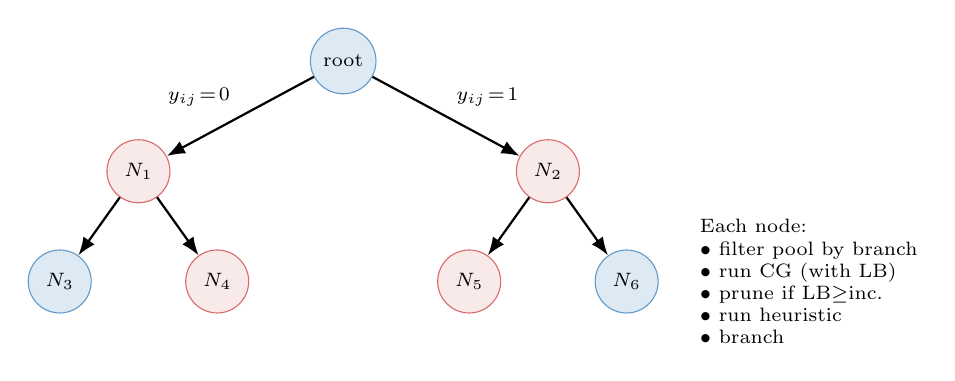
\begin{tikzpicture}[every node/.style={font=\scriptsize}]
   \tikzstyle{n}=[circle,draw,minimum size=8mm, fill=accent!10, draw=accent!70];
   \tikzstyle{nc}=[circle,draw,minimum size=8mm, fill=accent2!15, draw=accent2!70];
   \tikzstyle{l}=[draw,-{Latex},thick];
   \node[nc] (r)        at (0,0)   {root};
   \node[n]  (a)        at (-2.6,-1.4) {$N_1$};
   \node[n]  (b)        at ( 2.6,-1.4) {$N_2$};
   \node[nc] (aa)       at (-3.6,-2.8) {$N_3$};
   \node[n]  (ab)       at (-1.6,-2.8) {$N_4$};
   \node[n]  (ba)       at ( 1.6,-2.8) {$N_5$};
   \node[nc] (bb)       at ( 3.6,-2.8) {$N_6$};
   \draw[l] (r) -- node[above left]{$y_{ij}\!=\!0$} (a);
   \draw[l] (r) -- node[above right]{$y_{ij}\!=\!1$} (b);
   \draw[l] (a) -- node[above left]{} (aa);
   \draw[l] (a) -- (ab);
   \draw[l] (b) -- (ba);
   \draw[l] (b) -- (bb);
   \node[right=4mm of bb,align=left,scale=1.0]
     {\scriptsize Each node:\\\scriptsize $\bullet$ filter pool by branch\\
      \scriptsize $\bullet$ run CG (with LB)\\
      \scriptsize $\bullet$ prune if LB$\ge$inc.\\
      \scriptsize $\bullet$ run heuristic\\
      \scriptsize $\bullet$ branch};
  \end{tikzpicture}
  \begin{itemize}\small
    \item Solid blue nodes = pruned by bound or integrality.
    \item Tree depth $\sim |\mathcal N|$ in the worst case but very rarely so
          in practice.
  \end{itemize}
\end{frame}

\begin{frame}{Branching strategy summary}
  \begin{tabular}{@{}p{0.30\textwidth}p{0.37\textwidth}p{0.30\textwidth}@{}}
    \toprule
    Rule & Pricing change & Use when \\
    \midrule
    Master $x_p$ (naive) & $k$-shortest path; bad & never \\
    Ryan-Foster (i,j) & merge / forbid pair & set-partitioning \\
    Arc $y_{uv}$ & remove / contract arc & VRP, network flow \\
    Resource $\tau_v$ & split window & deep nodes \\
    Aggregated knapsack & on $a_{ip}$-vector & cutting stock \\
    \bottomrule
  \end{tabular}
  \medskip
  \begin{keybox}[Lab choice]
    We'll implement \alert{arc branching} -- one branch per fractional arc.
    Easy to apply, easy to filter the column pool by ``does the route use
    arc $(u,v)$''.
  \end{keybox}
\end{frame}

\begin{frame}{\textbf{[lab]} Exercise E -- B\&P with Lagrangian pruning}
  \begin{exbox}[Exercise E -- arc-branching B\&P]
    \begin{itemize}\small
      \item Implement
            \texttt{lagrangian\_bound(mp\_dual\_by\_id, pricing\_sols, K)}
            -- formula on the next slide. The B\&P engine uses this to prune.
      \item Write
            \texttt{aggregated\_arc\_flow}: $\bar y_{uv}\!=\!\sum_{p:(u,v)\in p}\bar x_p$.
      \item Pick the most-fractional arc; build the two children
            (\texttt{forbid} / \texttt{force}). Implement the
            pricing-graph edit (\texttt{EX-E.5}: skip forbidden arcs).
      \item Filter the parent column pool: drop columns incompatible with
            the branch; keep the rest as warm-start.
    \end{itemize}
    The B\&P loop itself is already coded in \texttt{bnp.py}; you fill
    only the helpers \texttt{EX-E.1, E.2, E.3, E.5}. The Lagrangian
    bound is reused from Exercise C / Trick~7. Knobs to play with at the
    end: \texttt{--gap} (stop within $\delta\%$),
    \texttt{--no-depth-first} (pure best-first),
    \texttt{--rmh-every} (heuristic frequency).

    \alert{Time budget: 35 minutes -- end-of-workshop deliverable.}
  \end{exbox}
\end{frame}

% =====================================================================
\section{Visualising convergence}
% =====================================================================

\begin{frame}{Seeing the algorithm}
  Two helpers ship with the lab kit (\texttt{vrp.plot}) and turn the
  CG / B\&P traces into \alert{convergence figures}:
  \begin{itemize}\small
    \item \texttt{plot\_cg\_convergence(runs)} -- LP \& LB per iteration
          plus the duality gap, for several CG configurations on the same
          axes. Powered by \texttt{CGStats.lp\_history},
          \texttt{CGStats.lb\_history} (filled by every CG call).
    \item \texttt{plot\_bnp\_progress(runs)} -- UB / LB and gap per
          \emph{node processed} (top row) and per \emph{wall-clock second}
          (bottom row), for several B\&P configurations.
          Powered by the \texttt{BnPIncumbent.\{ub,lb,time\}\_history}
          fields that the B\&P engine records as it goes.
  \end{itemize}
  \begin{keybox}[Why look at the curves]
    Picking K, $\alpha$, gap and search order from a table of final
    numbers misses the dynamics. The convergence curves show
    \emph{when} each parameter pays off (early vs late) and reveal
    tailing-off vs sustained progress.
  \end{keybox}
\end{frame}

\begin{frame}[fragile]{Comparison runners}
\begin{lstlisting}[language=bash]
# CG -- batch sizes
python -m vrp.tests.compare_cg --instance RC101.txt --nb-cols-list 1 5 20 50

# CG -- Wentges smoothing
python -m vrp.tests.compare_cg --instance RC101.txt --alphas 0 0.2 0.5

# B&P -- gap thresholds
python -m vrp.tests.compare_bnp --instance R101.txt --gaps 0 2 5

# B&P -- depth-first vs best-first
python -m vrp.tests.compare_bnp --instance R101.txt --search both

# B&P -- pricing batch sizes
python -m vrp.tests.compare_bnp --instance R101.txt --nb-cols-list 5 20 50
\end{lstlisting}
  Add \texttt{--save figure.png} to write the figure to disk instead of
  displaying it. Every CG / B\&P run inside the comparison uses the
  same logger, so \texttt{-v} also pours iteration logs to stderr.
\end{frame}

\begin{frame}{What the experiments tell you}
  \begin{itemize}\setlength{\itemsep}{4pt}
    \item \textbf{K vs iterations} -- $K\!=\!1$ takes many iterations but
          each is cheap; $K\!=\!50$ takes few iterations but each LP is
          heavier. Expect the wall-clock curve to be U-shaped.
    \item \textbf{Wentges $\alpha$} -- $\alpha\!\in\![0.3,0.7]$ usually
          halves iterations on Solomon-100. Too high ($\alpha\!=\!0.9$)
          makes LB lag, hurting the gap-stop.
    \item \textbf{Gap stop} -- on R101, \texttt{gap=2\%} typically closes
          80\% of the optimality gap in 20\% of the time.
    \item \textbf{Depth-first vs best-first} -- depth-first finds an
          incumbent faster (good for pruning); best-first closes the
          \alert{global LB} faster (good when you want a small certified
          gap). Hybrid solvers do both.
  \end{itemize}
\end{frame}

\begin{frame}{Hand-off to the lab}
  \begin{itemize}\small
    \item All five exercises (A--E) are in the \alert{lab kit}
          (\texttt{python/}), with a per-exercise check script and
          a reference solution under \texttt{solutions/}.
    \item The lab deck (\texttt{lab.pdf}) walks you through installation,
          file map, expected outputs and the optional comparison runners
          (\texttt{compare\_cg}, \texttt{compare\_bnp}).
    \item Every step logs to \texttt{stderr} via the \texttt{vrp.log}
          module; \texttt{-v} switches to \texttt{DEBUG}. B\&P lines are
          colour-tagged so the tree progress stands out at a glance.
  \end{itemize}
\end{frame}

% =====================================================================
\section{Recap and references}
% =====================================================================

\begin{frame}{Recap -- what we covered}
  \begin{itemize}\small
    \item \textbf{Why}: extended formulations with one variable per
          combinatorial object beat compact LPs.
    \item \textbf{How}: solve the restricted master, compute duals, price
          new columns, repeat.
    \item \textbf{Pricer}: RCSPP via label-setting; resources, dominance,
          ng-routes, multi-column return.
    \item \textbf{Speed}: stabilisation, hierarchy of pricers, warm-start
          LP, column pool management, tailing-off.
    \item \textbf{Integrality}: RMH, diving, price-and-branch.
    \item \textbf{Optimality}: branch-and-price, smart branching rules,
          Lagrangian bound for early pruning.
  \end{itemize}
\end{frame}

\begin{frame}{Recap -- one diagram}
  \begin{center}
  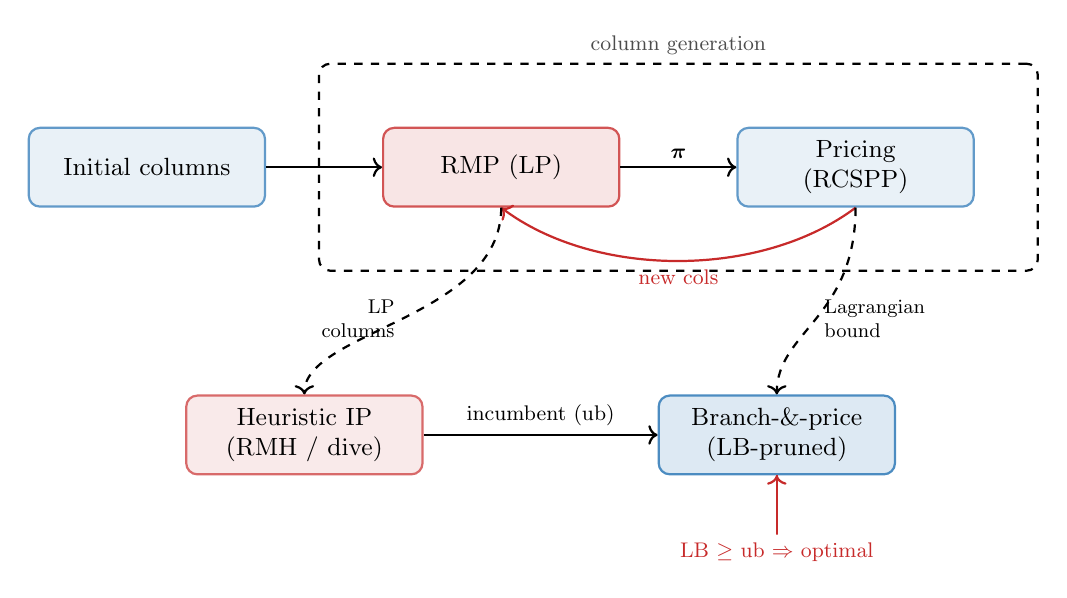
\begin{tikzpicture}[every node/.style={font=\small}]
    \tikzstyle{p}=[rounded corners,draw,minimum width=30mm,minimum height=10mm,
                   align=center,thick];
    \tikzstyle{loop}=[draw,rounded corners,thick,dashed,inner sep=4mm];

    % top row: CG loop
    \node[p,fill=accent2!10,draw=accent2!70] (init)  at (0,0)    {Initial columns};
    \node[p,fill=accent!12,draw=accent!80]   (rmp)   at (4.5,0)  {RMP (LP)};
    \node[p,fill=accent2!10,draw=accent2!70] (price) at (9.0,0)  {Pricing\\(RCSPP)};
    \draw[->,thick] (init) -- (rmp);
    \draw[->,thick] (rmp.east) -- node[above,scale=0.85]{$\boldsymbol\pi$} (price.west);
    \draw[->,thick,accent] (price.south) .. controls +(-1.2,-0.9) and +(1.2,-0.9) ..
       node[below,scale=0.85,align=center]{new cols} (rmp.south);
    \node[loop,fit=(rmp)(price),inner sep=8mm,label={[scale=0.85,gray!60!black]above:column generation}] {};

    % bottom row: integer
    \node[p,fill=accent!10,draw=accent!70]   (heur)  at (2.0,-3.4) {Heuristic IP\\(RMH / dive)};
    \node[p,fill=accent2!15,draw=accent2!80] (bp)    at (8.0,-3.4) {Branch-\&-price\\(LB-pruned)};

    \draw[->,thick,dashed] (rmp.south)  ..  controls +(0,-1.4) and +(0,0.8) ..
       node[left,scale=0.8,align=right]{LP\\columns}   (heur.north);
    \draw[->,thick,dashed] (price.south)  ..  controls +(0,-1.4) and +(0,0.8) ..
       node[right,scale=0.8,align=left]{Lagrangian\\bound}                (bp.north);
    \draw[->,thick] (heur.east) -- node[above,scale=0.85]{incumbent (ub)} (bp.west);
    \draw[->,thick,accent] (bp.south) .. controls +(0,-1.0) and +(0,-1.0) ..
       node[below,scale=0.85,align=center]{LB $\ge$ ub $\Rightarrow$ optimal} (bp.south);
  \end{tikzpicture}
  \end{center}
\end{frame}

\begin{frame}{If you remember three things}
  \begin{enumerate}\setlength{\itemsep}{6pt}
    \item \textbf{Don't enumerate}: the master never sees most of $\mathcal P$.
          You generate columns only when their reduced cost is negative.
    \item \textbf{Branch on structure, not on master variables}: Ryan-Foster,
          arc branching, resource branching all keep the pricing problem
          intact.
    \item \textbf{The Lagrangian bound is your friend}: it converts a
          fractional LP into a true lower bound, kills CG tailing-off, and
          prunes B\&P nodes early.
  \end{enumerate}
\end{frame}

\begin{frame}{References (1/3) -- foundations}
  \scriptsize
  \begin{itemize}\setlength{\itemsep}{2pt}
    \item P.~Gilmore \& R.~Gomory, \emph{A linear programming approach to the
          cutting stock problem}, Operations Research, 9(6), 849--859, 1961.
    \item G.~Dantzig \& P.~Wolfe, \emph{Decomposition principle for linear
          programs}, Operations Research, 8(1), 101--111, 1960.
    \item L.~Lasdon, \emph{Optimization theory for large systems},
          Macmillan, 1970 (Lagrangian bound).
    \item D.~Ryan \& B.~Foster, \emph{An integer programming approach to
          scheduling}, in Computer Scheduling of Public Transport
          (A.~Wren, ed.), 269--280, North-Holland, 1981.
    \item M.~Desrochers \& F.~Soumis, \emph{A generalized permanent labelling
          algorithm for the shortest path problem with time windows},
          INFOR, 26(3), 191--212, 1988.
    \item C.~Barnhart, E.~Johnson, G.~Nemhauser, M.~Savelsbergh \& P.~Vance,
          \emph{Branch-and-price: column generation for solving huge integer
          programs}, Operations Research, 46(3), 316--329, 1998.
    \item J.~Desrosiers, F.~Soumis \& M.~Desrochers, \emph{Routing with time
          windows by column generation}, Networks, 14(4), 545--565, 1984.
  \end{itemize}
\end{frame}

\begin{frame}{References (2/3) -- methods \& algorithms}
  \scriptsize
  \begin{itemize}\setlength{\itemsep}{2pt}
    \item O.~du~Merle, D.~Villeneuve, J.~Desrosiers \& P.~Hansen,
          \emph{Stabilized column generation}, Discrete Mathematics,
          194(1-3), 229--237, 1999.
    \item P.~Wentges, \emph{Weighted Dantzig--Wolfe decomposition for linear
          mixed-integer programming}, International Transactions in
          Operational Research, 4(2), 151--162, 1997 (smoothing).
    \item F.~Vanderbeck, \emph{Implementing mixed integer column generation},
          in Column Generation (G.~Desaulniers, J.~Desrosiers \& M.M.~Solomon,
          eds.), 331--358, Springer, 2005.
    \item F.~Vanderbeck \& L.A.~Wolsey, \emph{Reformulation and decomposition
          of integer programs}, in 50 Years of Integer Programming, 431--502,
          Springer, 2010.
    \item R.~Baldacci, A.~Mingozzi \& R.~Roberti, \emph{New route relaxation
          and pricing strategies for the VRPTW}, Operations Research,
          59(5), 1269--1283, 2011 (ng-routes).
    \item D.~Pecin, A.~Pessoa, M.~Poggi \& E.~Uchoa, \emph{Improved
          branch-cut-and-price for capacitated vehicle routing}, Mathematical
          Programming Computation, 9(1), 61--100, 2017 (subset-row cuts).
    \item N.~Boland, J.~Dethridge \& I.~Dumitrescu, \emph{Accelerated
          label-setting algorithms for the elementary RCSPP}, Operations
          Research Letters, 34(1), 58--68, 2006 (bidirectional pricing).
  \end{itemize}
\end{frame}

\begin{frame}{References (3/3) -- workshop pointers}
  \scriptsize
  \begin{itemize}\setlength{\itemsep}{2pt}
    \item J.~Desrosiers, M.~L\"ubbecke, G.~Desaulniers \& J.B.~Gauthier,
          \emph{Branch-and-Price}, Springer, 2026 (open access).
          ISBN 978-3-031-96917-1, DOI \texttt{10.1007/978-3-031-96917-1}
          (PDF in your workshop folder).
    \item G.~Desaulniers, J.~Desrosiers \& M.M.~Solomon (eds.),
          \emph{Column Generation}, Springer, 2005.
    \item M.M.~Solomon, \emph{Algorithms for the vehicle routing and
          scheduling problems with time window constraints}, Operations
          Research, 35(2), 254--265, 1987 (the benchmark instances we use).
    \item Open-source LP/MIP: HiGHS (\url{https://highs.dev}); CBC, GLPK.
    \item Research B\&P solvers: BaPCod, GCG, VRPSolver, RouteOpt.
    \item Python ecosystem: \texttt{rcspp} (workshop), \texttt{highspy},
          \texttt{pulp}, \texttt{coptpy}, \texttt{networkx}.
  \end{itemize}
\end{frame}

\begin{frame}{Hand-off to the lab kit}
  \begin{center}
    \large
    The hands-on companion deck (\texttt{lab.pdf}) walks you through:\\[0.6em]
  \end{center}
  \begin{itemize}\small
    \item installation (Python, virtualenv, HiGHS, \texttt{rcspp});
    \item the directory layout of the \texttt{python/} folder;
    \item how to run the smoke test, then exercises A through E;
    \item expected outputs and common pitfalls.
  \end{itemize}
  \vfill
  \centering Good luck -- and break the LP, not the dominance!
\end{frame}

\end{document}
